\documentclass[12pt,twoside]{report}

%\usepackage{todonotes}

%\usepackage{ifthen}
\usepackage{amssymb}
\usepackage{ulem}
\usepackage{xcolor}

% Document Configuration
%%%%%%%%%%%%%%%%%%%%%%%%%%%%%%%%%%%%%%%%%%%%%%%%%%%%%%%%%%%%%%%%%%%%%%

\usepackage{tabularx}
\usepackage{longtable}
\usepackage{ltxtable}
\usepackage{booktabs}
\usepackage{array}
\usepackage{collcell}
\usepackage{trimspaces}
\usepackage{multirow}
\usepackage{rotating}

%%%
%%% Formatting
%%%

% New rule type
\newcommand{\topruleb}{\midrule[\heavyrulewidth]}

% Commands to control the alignment of headers
\newcommand{\bfu}[1]{\textbf{\uppercase{#1}}}
\newcommand{\headingl}[1]{\multicolumn{1}{l}{\bfu{#1}}}
\newcommand{\headingc}[1]{\multicolumn{1}{c}{\bfu{#1}}}
\newcommand{\headingr}[1]{\multicolumn{1}{r}{\bfu{#1}}}

% Regular column types
\newcolumntype{x}{>{\collectcell\textsc}l<{\endcollectcell}}
\newcolumntype{y}{>{\collectcell\textsc}c<{\endcollectcell}}
\newcolumntype{z}{>{\collectcell\textsc}r<{\endcollectcell}}
\newcolumntype{u}{>{\collectcell\uppercase}l<{\endcollectcell}}
\newcolumntype{v}{>{\collectcell\uppercase}c<{\endcollectcell}}
\newcolumntype{w}{>{\collectcell\uppercase}r<{\endcollectcell}}
\newcolumntype{U}{>{\bfseries\collectcell\uppercase}l<{\endcollectcell}}
\newcolumntype{V}{>{\bfseries\collectcell\uppercase}c<{\endcollectcell}}
\newcolumntype{W}{>{\bfseries\collectcell\uppercase}r<{\endcollectcell}}

% Paragraph column types
\newcolumntype{L}{>{\raggedright\arraybackslash}X}
\newcolumntype{C}{>{\centering\arraybackslash}X}
\newcolumntype{R}{>{\raggedleft\arraybackslash}X}

\usepackage{xspace}
\usepackage{lipsum}
\usepackage{xcolor}

% Short verbatim can be formatted using \!text!: e.g., \!boolean!
\def\!#1!{\texttt{#1}}

% Acronyms should be placed in angled brackets: e.g., \<UML>
\def\<#1>{\lowercase{\textsc{#1}}}

% Abbreviations for references
\newcommand{\Figure}{Figure\@\xspace}
\newcommand{\Figures}{Figures\@\xspace}
\newcommand{\Table}{Table\@\xspace}
\newcommand{\Tables}{Tables\@\xspace}
\newcommand{\Section}{Section\@\xspace}
\newcommand{\Sections}{Sections\@\xspace}
\newcommand{\Appendix}{Appendix\@\xspace}
\newcommand{\Appendices}{Appendices\@\xspace}


% Common abbrev. are set as commands to ensure proper spacing after the dot
\newcommand{\ie}{i.e.\@\xspace}
\newcommand{\Ie}{I.e.\@\xspace}
\newcommand{\cf}{cf.\@\xspace}
\newcommand{\Cf}{Cf.\@\xspace}
\newcommand{\eg}{e.g.\@\xspace}
\newcommand{\Eg}{E.g.\@\xspace}
\newcommand{\etal}{et al.\@\xspace}
\newcommand{\etc}{etc.\@\xspace}

% Sample text
%\newcommand{\stext}[1][1-2]{\textcolor{gray!80!red}{\lipsum[#1]}}
\newcommand{\stext}[1][1-2]{\lipsum[#1]}

% Sample paragraph
\newcommand{\spar}{\stext[1]}

% Short sample paragraph
\newcommand{\sspar}{\stext[66]}
\usepackage{enumitem}
\usepackage{relsize}
\usepackage{textcomp}
\usepackage{rotating}
\usepackage{graphbox}
\usepackage{float}
\usepackage{xfrac}
\usepackage{placeins}
\usepackage{subcaption}
\usepackage[numbers,sort]{natbib}

\usepackage{acronym}
\renewcommand*{\aclabelfont}[1]{\textcolor{blue}{#1}}
%\renewcommand*{\acsfont}[1]{\textsc{#1}}

\usepackage{url}
% Allow breaking URLs at any character
\expandafter\def\expandafter\UrlBreaks\expandafter{\UrlBreaks%
  \do\a\do\b\do\c\do\d\do\e\do\f\do\g\do\h\do\i\do\j%
  \do\k\do\l\do\m\do\n\do\o\do\p\do\q\do\r\do\s\do\t%
  \do\u\do\v\do\w\do\x\do\y\do\z\do\A\do\B\do\C\do\D%
  \do\E\do\F\do\G\do\H\do\I\do\J\do\K\do\L\do\M\do\N%
  \do\O\do\P\do\Q\do\R\do\S\do\T\do\U\do\V\do\W\do\X%
  \do\Y\do\Z}

% Allow hyphenation in texttt
\LetLtxMacro\origttfamily\ttfamily
\DeclareRobustCommand*{\ttfamily}{%
  \origttfamily
  \hyphenchar\font=`\-\relax
  \fontdimen3\font=.25em\relax
  \fontdimen4\font=.167em\relax
  \fontdimen7\font=.167em\relax
}
%\usepackage{tikz}
\usetikzlibrary{arrows}
\usetikzlibrary{shapes}
\usetikzlibrary{patterns}
\usetikzlibrary{positioning}
\usetikzlibrary{calc}
\usetikzlibrary{trees}

\newcommand*{\stereotype}[1]{
  <<{#1}>>
}

\newcommand*{\datatype}[1]{
  \stereotype{datatype}\\
  #1
}

\newcommand*{\enum}[1]{
  \stereotype{enumeration}\\
  #1
}

\newcommand*{\obj}[2]{
  \underline{{#1}~:~{#2}}
}

\newcommand*{\attributes}[1]{
  \nodepart{second}
  \begin{tabular}{@{}l@{}}
  #1
  \end{tabular}
}

\newcommand*{\literals}[1]{
  \nodepart{second}
  \ttfamily
  \begin{tabular}{@{}l@{}}
  #1
  \end{tabular}
}

\newcommand*{\operations}[1]{
  \nodepart{third}
  \begin{tabular}{@{}l@{}}
  #1
  \end{tabular}
}

\tikzstyle{reportcolor}=[
  draw=black,
  line width = 0.4pt
]

\tikzstyle{box}=[
  reportcolor,
  rectangle,
  align=center,
  minimum width=5em
]

\tikzstyle{abstractbox}=[box,
  every text node part/.style={
    font=\itshape
  }
]

\tikzstyle{class}=[box,
  rectangle split,
  rectangle split parts=2,
  minimum width=9em,
  rectangle split part align={center, left}
]

\tikzstyle{classop}=[class,
  rectangle split parts=3,
  rectangle split part align={center, left, left}
]
  
\tikzstyle{object}=[class]

\tikzstyle{abstractclass}=[class,
  every text node part/.style={
    font=\itshape
  }
]

\tikzstyle{enum}=[class]

\tikzstyle{datatype}=[class]

\tikzstyle{inherits}=[reportcolor, ->, > = open triangle 90]

\tikzstyle{contains}=[reportcolor, diamond->, > = angle 45]

\tikzstyle{assoc}=[reportcolor, ->, > = angle 45]

\tikzstyle{biassoc}=[reportcolor, <->, > = angle 45]


 
\usepackage{xcolor}
\usepackage{ifthen}
\usepackage{amssymb}
\usepackage{tabto}
\usepackage[page]{pagenote}
\makepagenote

\newlength\cindent
\setlength\cindent{1.5em}
\renewcommand{\notesname}{\uppercase{Notes for Clarifications}}
\renewcommand*{\notedivision}{\section*{\notesname}}
\renewcommand*{\sectionname}{\uppercase{Section}}
\renewcommand{\notenumintext}[1]{\textsuperscript{\textcolor{red}{#1}}}
\renewcommand{\thepagenote}{\roman{pagenote}}
\renewcommand{\prenoteinnotes}{\par\hangindent=\cindent\hangafter=1\noindent}
\renewcommand{\postnoteinnotes}{\par}
\renewcommand{\noteentry}[4]{%
\prenoteinnotes
\noteidinnotes{#1}{#2}%
\tabto{\cindent}%
\noteinnotes{#3}\dotfill%
\textcolor{blue}{\pageinnotes{#4}}%
\vspace{6pt}
\postnoteinnotes}

\makeatletter
\def\blankfootnote{\xdef\@thefnmark{}\@footnotetext}
\makeatother



\newcommand{\clarify}[2]{%
  {\color{red}%
      #1%
    \ifthenelse{\equal{#2}{}}{%
    }{%
      \addtocounter{pagenote}{1}%
      \blankfootnote{\color{red}\textsuperscript{\thepagenote}~#2}%
      \addtocounter{pagenote}{-1}%
    }%
  }%
  \ifthenelse{\equal{#1}{}}{%
    \ifthenelse{\equal{#2}{}}{%
    }{%
      \pagenote{#2}%
    }%
  }{%
    \ifthenelse{\equal{#2}{}}{%
      \pagenote{\textcolor{blue}{#1}}%
    }{%
      \pagenote{\textcolor{blue}{#1} --- #2}%
    }%
  }%
} 

%For code listings:
\usepackage{listings}
\usepackage{parcolumns}


\definecolor{gray97}{gray}{.97}
\definecolor{gray75}{gray}{.75}
\definecolor{gray45}{gray}{.45}
\definecolor{gray20}{gray}{.20}

\definecolor{codeblue}{rgb}{0.2,0.6,.6}
\definecolor{codegreen}{rgb}{0,0.6,0}
\definecolor{codegray}{rgb}{0.5,0.5,0.5}
\definecolor{codepurple}{rgb}{0.58,0,0.82}
\definecolor{backcolour}{rgb}{0.95,0.95,0.92}



\lstdefinestyle{mystyle}{
    backgroundcolor=\color{backcolour},   
    commentstyle=\color{codegreen},
    keywordstyle=\color{black}\textbf,
    numberstyle=\tiny\color{codegray},
    stringstyle=\color{codepurple},
    basicstyle=\footnotesize,
    breakatwhitespace=false,         
    breaklines=true,                 
    captionpos=b,                    
    keepspaces=true,                 
    numbers=left,                    
    numbersep=5pt,                  
    showspaces=false,                
    showstringspaces=false,
    showtabs=false,                  
    tabsize=2,
    morekeywords={confidences,artefacts,fragments,relationshiptypes,relationshiptype,DomainType,EngineeringType,Trace,tracelinks,NodeTraceLink,LeafTraceLink,source,target,successors,referee,confidence,agents,HumanAgent,MachineAgent,Confidence,value,evidences,AIEvidence,agency,algorithmUsed,parameters,executionDate,trainingResults,impactedElements}
}
\lstdefinestyle{mystylesysml}{
    backgroundcolor=\color{backcolour},   
    commentstyle=\color{codepurple}\textit,
    morecomment=[s][\color{codegreen}]{/**}{*/},
    morecomment=[s][\color{codegreen}]{/*}{*/},
    keywordstyle=\color{codepurple}\textbf,
    numberstyle=\tiny\color{codegray},
    stringstyle=\color{codegray},
    basicstyle=\footnotesize,
    breakatwhitespace=false,         
    breaklines=true,                 
    captionpos=b,                    
    keepspaces=true,                 
    numbers=left,                    
    numbersep=5pt,                  
    showspaces=false,                
    showstringspaces=false,
    showtabs=false,                  
    tabsize=2,
    linewidth=14cm,
    xleftmargin=4.2cm,
    frame=shadowbox,
    rulesepcolor=\color{blue},
   morekeywords={confidences,artefacts,fragments,relationshiptypes,relationshiptype,Trace,tracelinks,NodeTraceLink,LeafTraceLink,source,target,successors,referee,agents,value,evidences,agency,algorithmUsed,parameters,executionDate,trainingResults,impactedElements,from,trace,class,feature,to,impacts,package,attribute,def,import,metadata,about,assert,constraint,connect,connection,to}
}


\lstdefinestyle{mystylexcore}{
    backgroundcolor=\color{backcolour},   
    commentstyle=\color{codegreen},
    keywordstyle=\color{codeblue}\textbf,
    numberstyle=\tiny\color{codegray},
    stringstyle=\color{codepurple},
    basicstyle=\footnotesize,
    breakatwhitespace=false,         
    breaklines=true,                 
    captionpos=b,                    
    keepspaces=true,                 
    numbers=left,                    
    numbersep=5pt,                  
    showspaces=false,                
    showstringspaces=false,
    showtabs=false,                  
    tabsize=2,
    morekeywords={class,contains,abstract,extends,\{,\},\[,\],refers,derived,String,get,int,double},
    linewidth=14.5cm,
    xleftmargin=2.3cm
}

\lstdefinestyle{mystyleocl}{
    backgroundcolor=\color{backcolour},   
    commentstyle=\color{codegreen},
    keywordstyle=\color{black}\textbf,
    numberstyle=\tiny\color{codegray},
    stringstyle=\color{codepurple},
    basicstyle=\ttfamily\footnotesize,
    breakatwhitespace=false,         
    breaklines=true,                 
    captionpos=b,                    
    keepspaces=true,                 
    numbers=left,                    
    numbersep=5pt,                  
    showspaces=false,                
    showstringspaces=false,
    showtabs=false,                  
    tabsize=2,
    morekeywords={context,inv,includesAll,collect,self}
}

\lstdefinestyle{mystylextext}{
    backgroundcolor=\color{backcolour},   
    commentstyle=\color{codegreen},
    keywordstyle=\color{black}\textbf,
    numberstyle=\tiny\color{codegray},
    stringstyle=\color{codepurple},
    basicstyle=\ttfamily\footnotesize,
    breakatwhitespace=false,         
    % breaklines=true,                 
    captionpos=b,                    
    keepspaces=true,                 
    numbers=left,                    
    numbersep=5pt,                  
    showspaces=false,                
    showstringspaces=false,
    showtabs=false,                  
    tabsize=2,
    morekeywords={context,inv,includesAll,collect,self},
    linewidth=14cm,
    xleftmargin=0cm
}



% Standard shortcuts
\newcommand{\eg}{\emph{e.g.,~}}							% exempli gratia (for the sake of example)
\newcommand{\ie}{\emph{i.e.,~}}							% id est (that is)
\newcommand{\Fig}[1]{Fig.~\ref{#1}}  			% choose Fig. or Figure, depending on the style
\newcommand{\Table}[1]{Table~\ref{#1}}	    % Table reference
\newcommand{\Sect}[1]{Section~\ref{#1}}	  % section name always with a capital S
\newcommand{\Model}[1]{\textsf{\small{#1}}} % name of any modeling artifact (e.g., formalism, model element, rule, ...)
\newcommand{\Code}[1]{\texttt{\small{#1}}}	% inline code
\providecommand{\e}[1]{\ensuremath{\times 10^{#1}}}	% scientific notation: x.10^y

%%%%%%%%%%%%%%%%%%%%%%%%%%%%%%%%%%%%%%%%%%%%%

% Shortcuts
\newcommand{\MOF}{\textsc{MOF}\xspace}
\newcommand{\ocl}{\textsc{OCL}\xspace}
\newcommand{\OCL}{\textsc{OCL}\xspace}
\newcommand{\nsga}{\textsc{NSGA-II}\xspace}
\newcommand{\MDE}{\textsc{MDE}\xspace}
\newcommand{\MT}{\textsc{MT}\xspace}
\newcommand{\WFR}{\textsc{WFR}\xspace}
\newcommand{\Ecore}{\textsc{Ecore}\xspace}
\newcommand{\OURNAME}{{our approach}\xspace}



\newcommand{\ra}{$\rightarrow$}
\newcommand{\la}{$\leftarrow$}
\newcommand{\ugh}[1]{\textcolor{red}{\uwave{#1}}} % please rephrase
\newcommand{\ins}[1]{\textcolor{blue}{\uline{#1}}} % please insert
\newcommand{\del}[1]{\textcolor{red}{\sout{#1}}} % please delete
\newcommand{\chg}[2]{\textcolor{red}{\sout{#1}}{\ra}\textcolor{blue}{\uline{#2}}} % please change
\newcommand{\move}[2]{\textcolor{blue}{\uwave{#1} (Move to #2)}} % please move


\newboolean{showcomments}
\setboolean{showcomments}{true} % toggle to show or hide comments
\ifthenelse{\boolean{showcomments}}
{\newcommand{\nb}[2]{
		\fcolorbox{gray}{yellow}{\bfseries\sffamily\scriptsize#1}
		{$\blacktriangleright$#2$\blacktriangleleft$}
	}
	\newcommand{\version}{\emph{\scriptsize$-$working$-$}}
}
{\newcommand{\nb}[2]{}
	\newcommand{\version}{}
}



\newcommand\eb[1]{\nb{EB}{\textcolor{red}{\textsl{#1}}}}
\newcommand\jc[1]{\nb{JC}{\textcolor{red}{\textsl{#1}}}}
\newcommand{\todo}[1]{\textbf{\textcolor{red}{TODO: #1}}}
\newcommand\syn[0]{\fcolorbox{gray}{green}{\bfseries\sffamily\scriptsize{SYN.}}}

\newcommand\bluefat[1]{$\blacktriangleright$\textcolor{blue}{\textit{#1}}$\blacktriangleleft$}
\newcommand\blue[1]{\textcolor{blue}{#1}}
\newcommand\red[1]{\textcolor{red}{#1}}

\makeatletter
\def\ughu{\bgroup \markoverwith{\lower3.5\p@\hbox{\sixly \textcolor{red}{\char58}}}\ULon}
\font\sixly=lasy6 % does not re-load if already loaded, so no memory problem.
\makeatother


\newcommand\missref[1]{\ughu{#1}~\ugh{[?]}}

% Document Configuration 
%%%%%%%%%%%%%%%%%%%%%%%%%%%%%%%%%%%%%%%%%%%%%%%%%%%%%%%%%%%%%%%%%%%%%%
\title{5\textsuperscript{th} Deliverable:\\Visualizable and propagable SysMLv2 traces for metadata analysis}

\author{
  Edouard R. Batot 
} 

\date{ 
  December 15, 2021
}

% Begin document
%%%%%%%%%%%%%%%%%%%%%%%%%%%%%%%%%%%%%%%%%%%%%%%%%%%%%%%%%%%%%%%%%%%%%%

\begin{document}

% Title page
\maketitle 

% \title{5\textsuperscript{th} Deliverable: \textbf{Propagating trustable traceability}}
\title{5\textsuperscript{th} Deliverable: \textbf{Visualizable and propagable SysMLv2 traces}}

% Table of Contents
\tableofcontents

% Contents
\cleardoublepage
\renewcommand{\sectionbreak}{}
%!TEX root = ../document.tex
\section*{List of Acronyms}
\begin{descriptioncompact}
    \item[UOC] {Fundacio per a la Universitat Oberta de Catalunya}
    \item[SOM] {Systems, Software and Models Lab}
    \item[CEA] {Commissariat à l'énergie atomique et aux énergie alternatives}
    \item[SST] {SysML v2 Submission Team}
    \item
    \item[MDE] {Model-Driven Engineering}
    \item[SysML-v2] {Systems Modeling Language (SysML®) v2}
    \item[KerML] {Kernel Modeling Language (KerML)}
\end{descriptioncompact}

\vspace{33em}
\listoffigures
\lstlistoflistings
\renewcommand{\sectionbreak}{\cleardoublepage}
\cleardoublepage


%\section*{Foreword}
%\begin{figure}[ht] 
%	
%	\centering
%	
\includegraphics[width=.7\linewidth]{images/citation-ermine.pdf}
%\end{figure}



\section{Introduction}\label{sect:intro}

\begin{enumerate}
    \item SysMLv2 related limitations
        \begin{itemize}
            \item Metadata feature library - a promising idea
            \item Model level expression - a (still) deceitful implementation
        \end{itemize}
    \item Data structure components
         \begin{enumerate}
            \item Concrete implementation
                \begin{itemize}
                    \item From SysMLv2 metadata library to JSon: extraction and re-injection of metadata
                    \item JSon variability : multi-types, multi end, multi AnnotatingFeatures \textit{et al.}
                \end{itemize}
            \item Conditions for use
               \begin{itemize}
                    \item Separated files
                    \item Named connections
                    \item Programmatic version
                \end{itemize}
        \end{enumerate}
   
    % \item Integration of Tracea into DSL (UCMIS)
    %   \begin{itemize}
    %         \item Reminder Tracea
    %         \item UCMIS integration of Trace\textit{a}
    %     \end{itemize}
    \item Syntax representation: JSon for all
        \begin{itemize}
            \item Raw base extraction
            \item Visualization using D3-JS
            \item Matrix view
        \end{itemize}
    \item Implementers' guide
        \begin{itemize}
            \item Impact analysis scenario
            \item Energy consumption scenario
            \item Toward multi criteria apprehension 
                \begin{itemize}
                    \item Multiplicity/cardinality decisions
                    \item Integration target.. THEIA ?
                \end{itemize}
        \end{itemize}
\end{enumerate}
% This document presents the integration of Trace\textit{a} \cite{batot2021-not-another-metamodel}, a language dedicated to traceability into the new release of SysML language.
% It is the continuation of deliverables 1, 2, and 3 of the Trace\textit{a} project\footnote{Trace\textit{a} is part of the Modelia intiative which aims at "Bringing artificial intelligence to the modeling world"\\ \url{https://modelia.eu/projects/}.}. The first deliverable introduces the conceptualization work (SoA) related to traceability (D1)~\cite{deliverable1}. The second presents the metamodel of a language dedicated to traceability (D2) that fills the gaps detected in the existing literature during D1~\cite{deliverable2}. The third deliverable shows the evaluation and integration of functionalities (confidence and evidence) in a software dedicated to traceability (D3)~\cite{deliverable3}.
% This report presents the integration of the concepts related to traceability developed during these first three deliverables within SysMLv2\footnote{We alternately use the names SysML and SysMLv2 to refer to SysMLv2. The distinction between the two as well as all documentation relating to KerML / SysMLv2 is available by following the link:\\ \url{https://github.com/Systems-Modeling}.}.

This document is organized as follows.
\Sect{sec:background}, first briefly introduces the language dedicated to traceability that we have developed as well as the KerML / SysMLv2 ecosystem on which we integrate it. This section also defines the high level needs for quality traceability.
\Sect{sec:strategies}, presents which elements of KerML / SysMLv2 languages are of interest and how we have adapted and used them through the different integration strategies considered.
We will detail our choices of architecture and implementation and the limits that we encountered in \Sect{sec:extension}\footnote{We are integrating Trace\textit{a} into SysMLv2 while it is being formalized by the SST.}.
Finally, we conclude this document in \Sect{sec:conclusion} before pointing at the resulting software artefacts and their examples of use in \Sect{sec:artefacts}.






% \begin{descriptioncompact}
%      \item[Suite de Tracea] Livrables, objectifs
     
%      \item[Besoins de SysML] Intérêt à intégré Tracea au nouveau standard 
%      - Limitations
%      - Niveau de priorité faible (retard de livraison)
     
%      \item[Stratégies explorées] Elements du noyau (cibles de la traçabilité)
%      \begin{itemize}
%          \item  \textbf{Approches naïves/intrusives:} Modifier les éléments du noyau - Nouveau type d'annotation)
%          \item \textbf{Approches orthogonales:} Nouvelle fonction annotatrice - Bibliothèque de fonctionnalités) 
%      \end{itemize}
% \end{descriptioncompact}





\section{SysMLv2 related decisions}

During this fifth deliverable we ran into the limitations pointed out in the fourth deliverable. In this section, we present these limitations. 


\subsection{Metadata feature library -- a promising idea}
\begin{figure}[ht] 
	\centering
	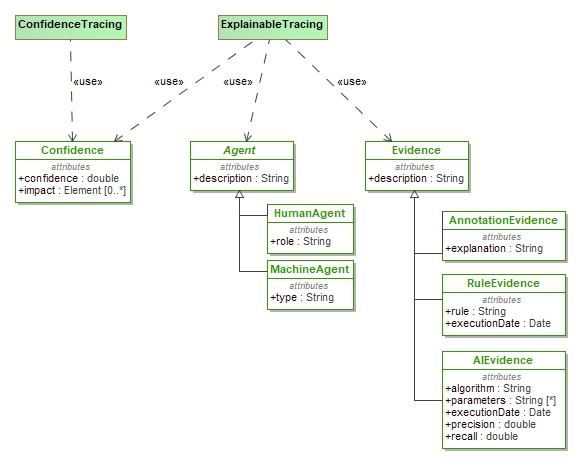
\includegraphics[width=.9\linewidth]{images/explainability-datatype.jpg}
	\caption{Metadatatypes for quality traceability including an assessment of confidence and monitoring of the identification processes used.}
	\label{fig:datatypes}
\end{figure}

% \vspace{3em}
The Listings \ref{lst:featurelibrary1} and \ref{lst:featurelibrary2} present our feature library {in SysML}. Listing~\ref{lst:featurelibrary1} contains the library declaration; Listing~\ref{lst:featurelibrary2} contains an example of application of such datatype  defined on a concrete example. It illustrates the allocation of a confidence value of 0.7 to a connection between a requirement (req) and a package. The second case (line 16 to 20) attributes a description and points to an element impacted (by the evaluation of the confidence),

% \vspace{10cm}

\begin{center}
\begin{lstlisting}[caption={Definition of a datatype dedicated to traceability (partial listing).},
label=lst:featurelibrary1,
style=mystylesysml,
linewidth=15cm,
xleftmargin=2.2cm,
morekeywords={part,filter}]
 package TracingAnnotations {
	attribute def ConfidenceTracing {
		attribute confidence : Real;
		attribute impact : Anything[*]
		assert constraint 
		  { confidence >= 0.0 && confidence <= 1.0 } 
	}
	 
	attribute def ExplainableTracing {
		attribute description : String;
		attribute evidence : Evidence;
		attribute agent : Agent;
	}  
 }
\end{lstlisting}
\end{center}  

\begin{center}
\begin{lstlisting}[caption={Use of metadata features for traceability},
label=lst:featurelibrary2,
style=mystylesysml,
frame=shadowbox,
rulesepcolor=\color{blue},
linewidth=15cm,
xleftmargin=2.2cm,
morekeywords={confidence,description,evidence,impact, part, req,package}]
 import package TracingAnnotations::*;

 /*Definition of the target system. */
 part vehiculetest {}
 req RE01_MLV {}
 package UMLCD_CORE {}

 /*Assignment of a confidence of 0.7 to the Req2Design link.*/
 connection Req2Design connect RE01_MLV to UMLCD_CORE {
   @ConfidenceTracing {
     confidence = 0.7;
   }
 }
 
 /*Assigning a description and an impact to the Req2Design link.*/
 connection Req2Design connect RE01_MLV to UMLCD_CORE {
   @ExplainableTracing {
     description = "Something";
     impact = (vehiculetest);
   }
 }
 
\end{lstlisting}
\end{center}


\subsection{Model level expression -- a deceitful implementation}
\begin{figure}[h]     
	\centering
	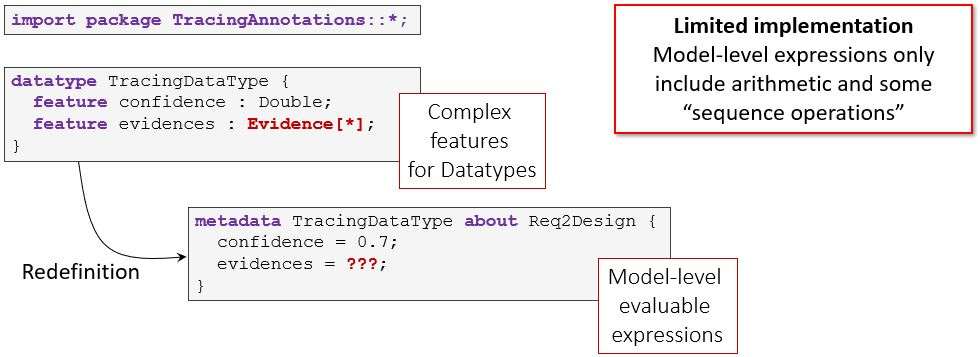
\includegraphics[width=.95\linewidth]{images/strategy4-metadatatype.jpg}
	\caption{Annotations and complex datatypes. }
	\label{fig:metadatatypes}
\end{figure}
When implementing these feature we ran into a number of disillusions. Fisrt and foremost, SysMLv2 implementation of the \textit{Model-level evaluable expressions} is for the least unsure. The concrete classes of the pilot implementation have been designed and written by only one developer (namely, Ed Seidewitz) and do not offer any safe guards. As showed in the previous deliverable, \Fig{fig:metadatatypes} points to where lies this limitation: when using a metadata feature, there is no guarantee for the use of "complex structures", \textit{i.e.,} that are not of basic types (int, double, String, ...). If used, these complex structure will at best show an error as pictured in \Fig{fig:filtererr}, and at worst keep the fallacious state of the system silent and leave the system out of its requirements.

\begin{figure}[ht]     
	\centering
	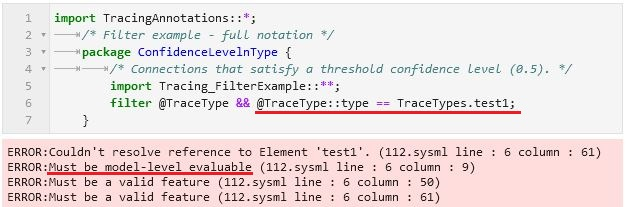
\includegraphics[width=.99\linewidth]{images/viz_filterexample_err.JPG}
	\caption{Limitation of the implementation of model-level evaluable expressions.}
	\label{fig:filtererr}
\end{figure}
\section{TraceaML support architecture}\label{sec:datastructure}
% \sideboxbegin{o}
% This section presents the limitation encountered while integrating the functionalities of Trace\textit{a} into SysMLv2.
% \sideboxend

This section introduces the decisions we made to activate Tracea's functionalities with SysMLv2 in its present state. We present the design decisions related to the traces and their trace links in a first place. Then we precise the conditions to the use of this implementation. 


\subsection{Decisions related to traceability features}
First, to overcome the limitations of the implementation of SysMLv2, we decided to concentrate on the use of basic types. These are sufficient to express the confidence degree, the types of traces and the (energy) cost attributed to a connection in the system.

Then, we had to choose between a certain number of options while implementing the features related to confidence and cost metadata. If confidence is a unique value for a link\footnote{We consider \textit{link} and \textit{connection} full synonym in this document.}, a link may have one or more source(s) and one or more target(s). As shown in For example, links may have one or more type(s). Yet, the visualization and semantics associated to such multi-valued attribute remains to discuss for annotating features do not restrict their usages. Since there is no way to restrict the definition of confidence annotations, what if more than one confidence is attributed to the same link? These variability points should be clearly and exhaustively understood to put our artefact to production. Meanwhile, multi-end and multi-typed links are allowed for persistence. Only the \textit{first} type and the first source and target are considered for the pilot visualization product.
\begin{figure}[h]     
	\centering
	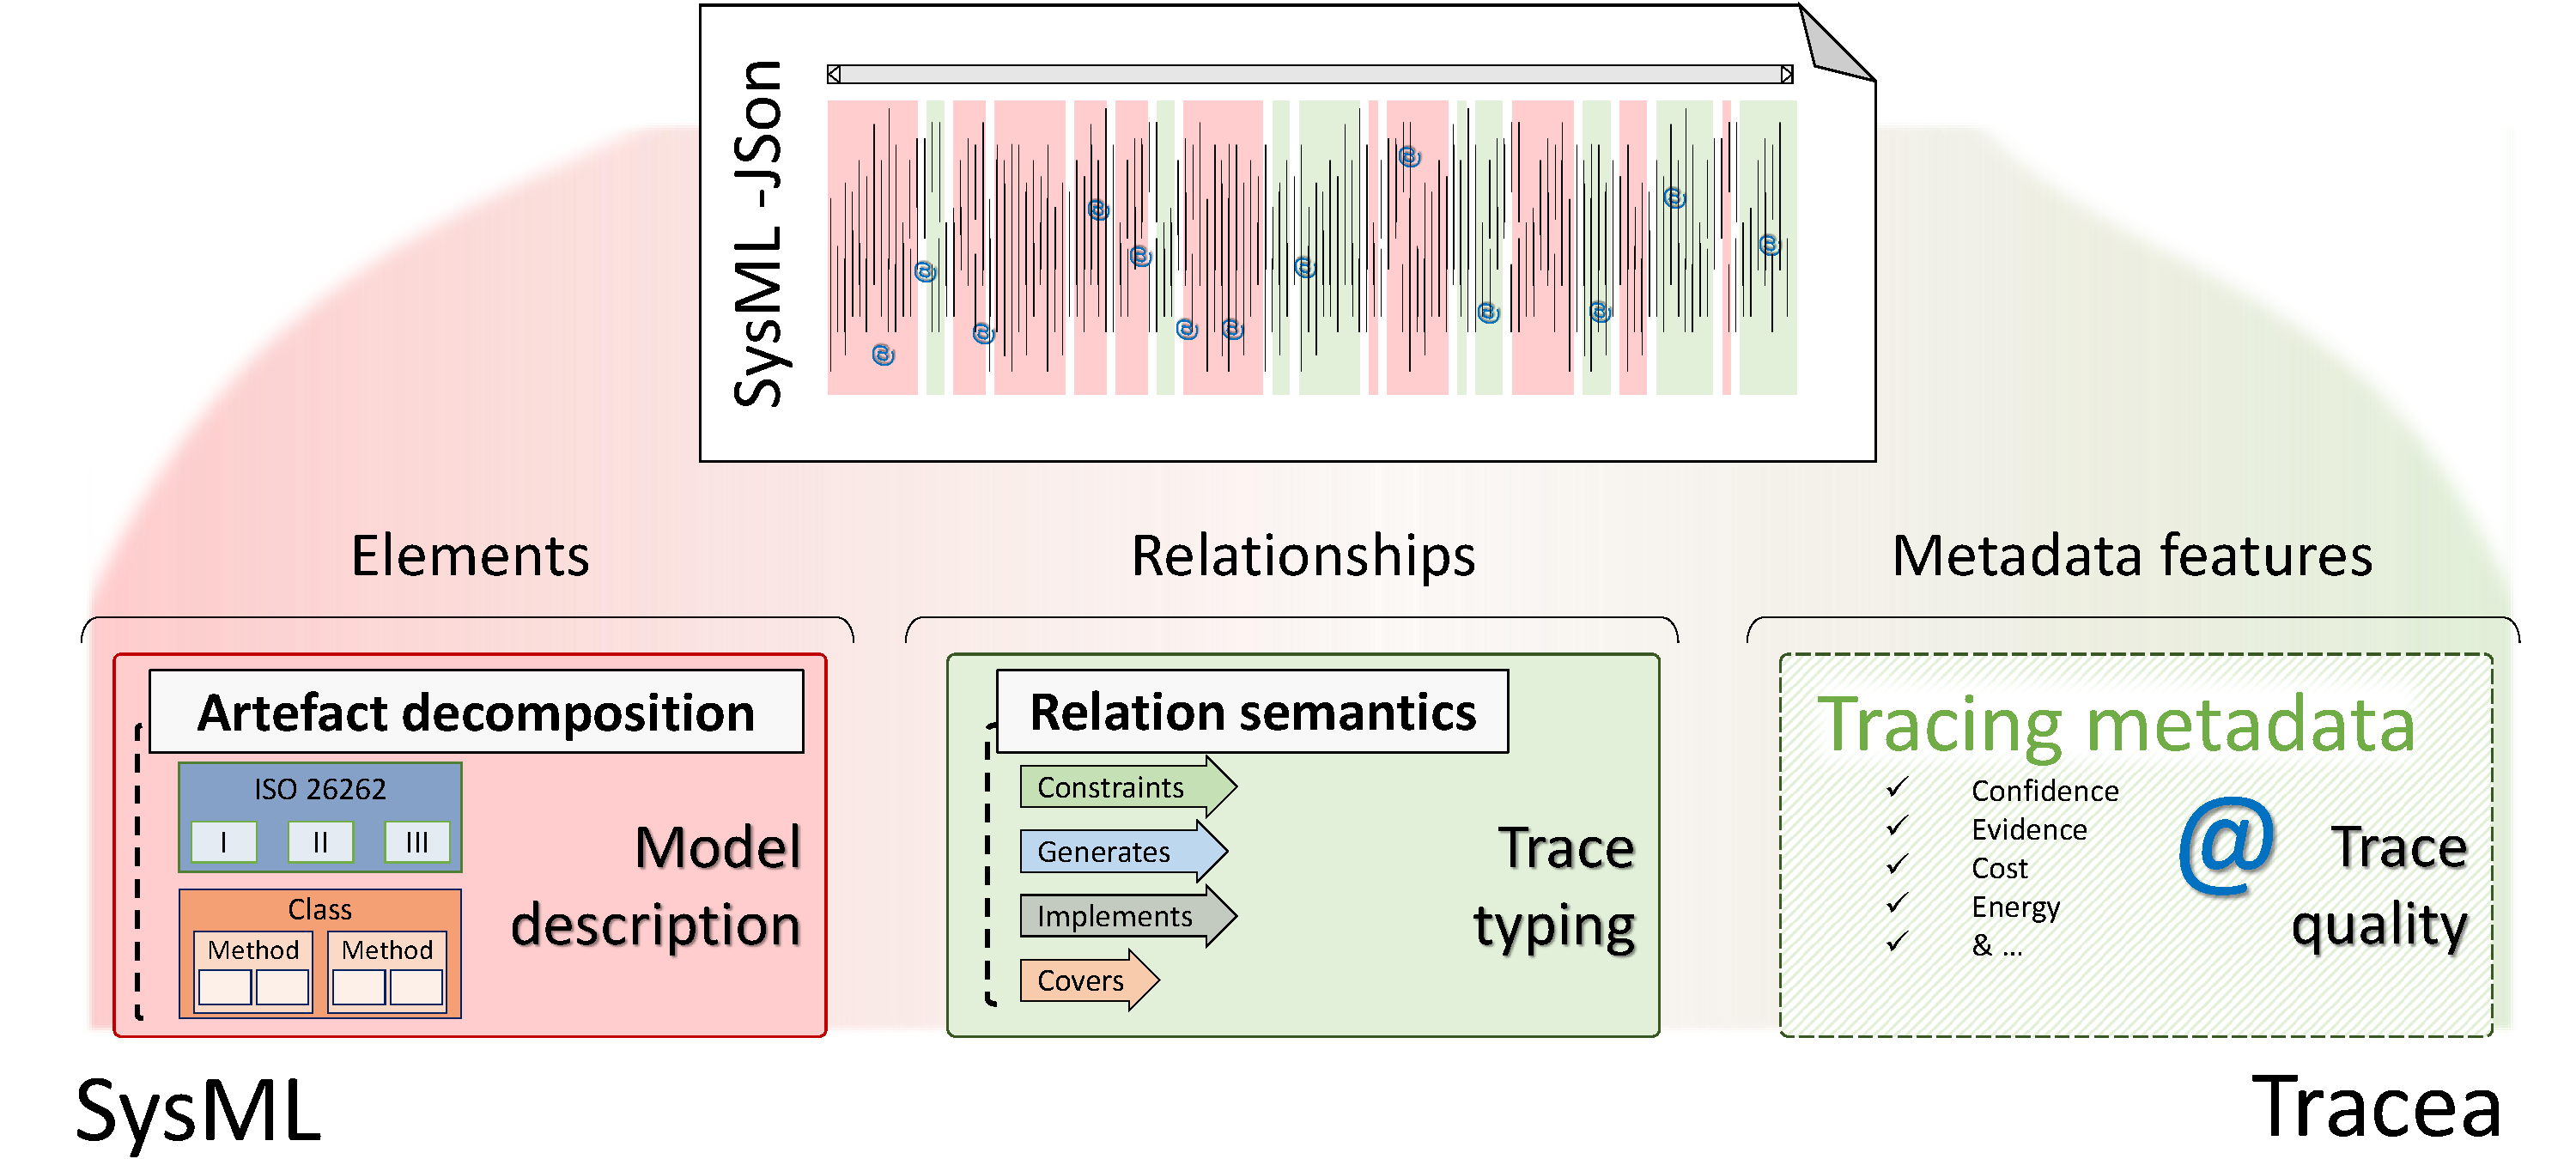
\includegraphics[width=.8\linewidth]{images/sysmljson-orga.pdf}
	\caption{Organisation of SysMLv2 JSon representation.}
	\label{fig:sysmljson-orga}
\end{figure}

% \begin{figure}[ht]     
% 	\centering
% 	\includegraphics[width=.7\linewidth]{images/cu-af-mf.jpg}
% 	\caption{Schematizing the multi-types conundrum.}
% 	\label{fig:multitypes}
% \end{figure}

\subsection{JSonTransformer: from SysMLv2 to TraceaML}
\begin{figure}[h]     
	\centering
	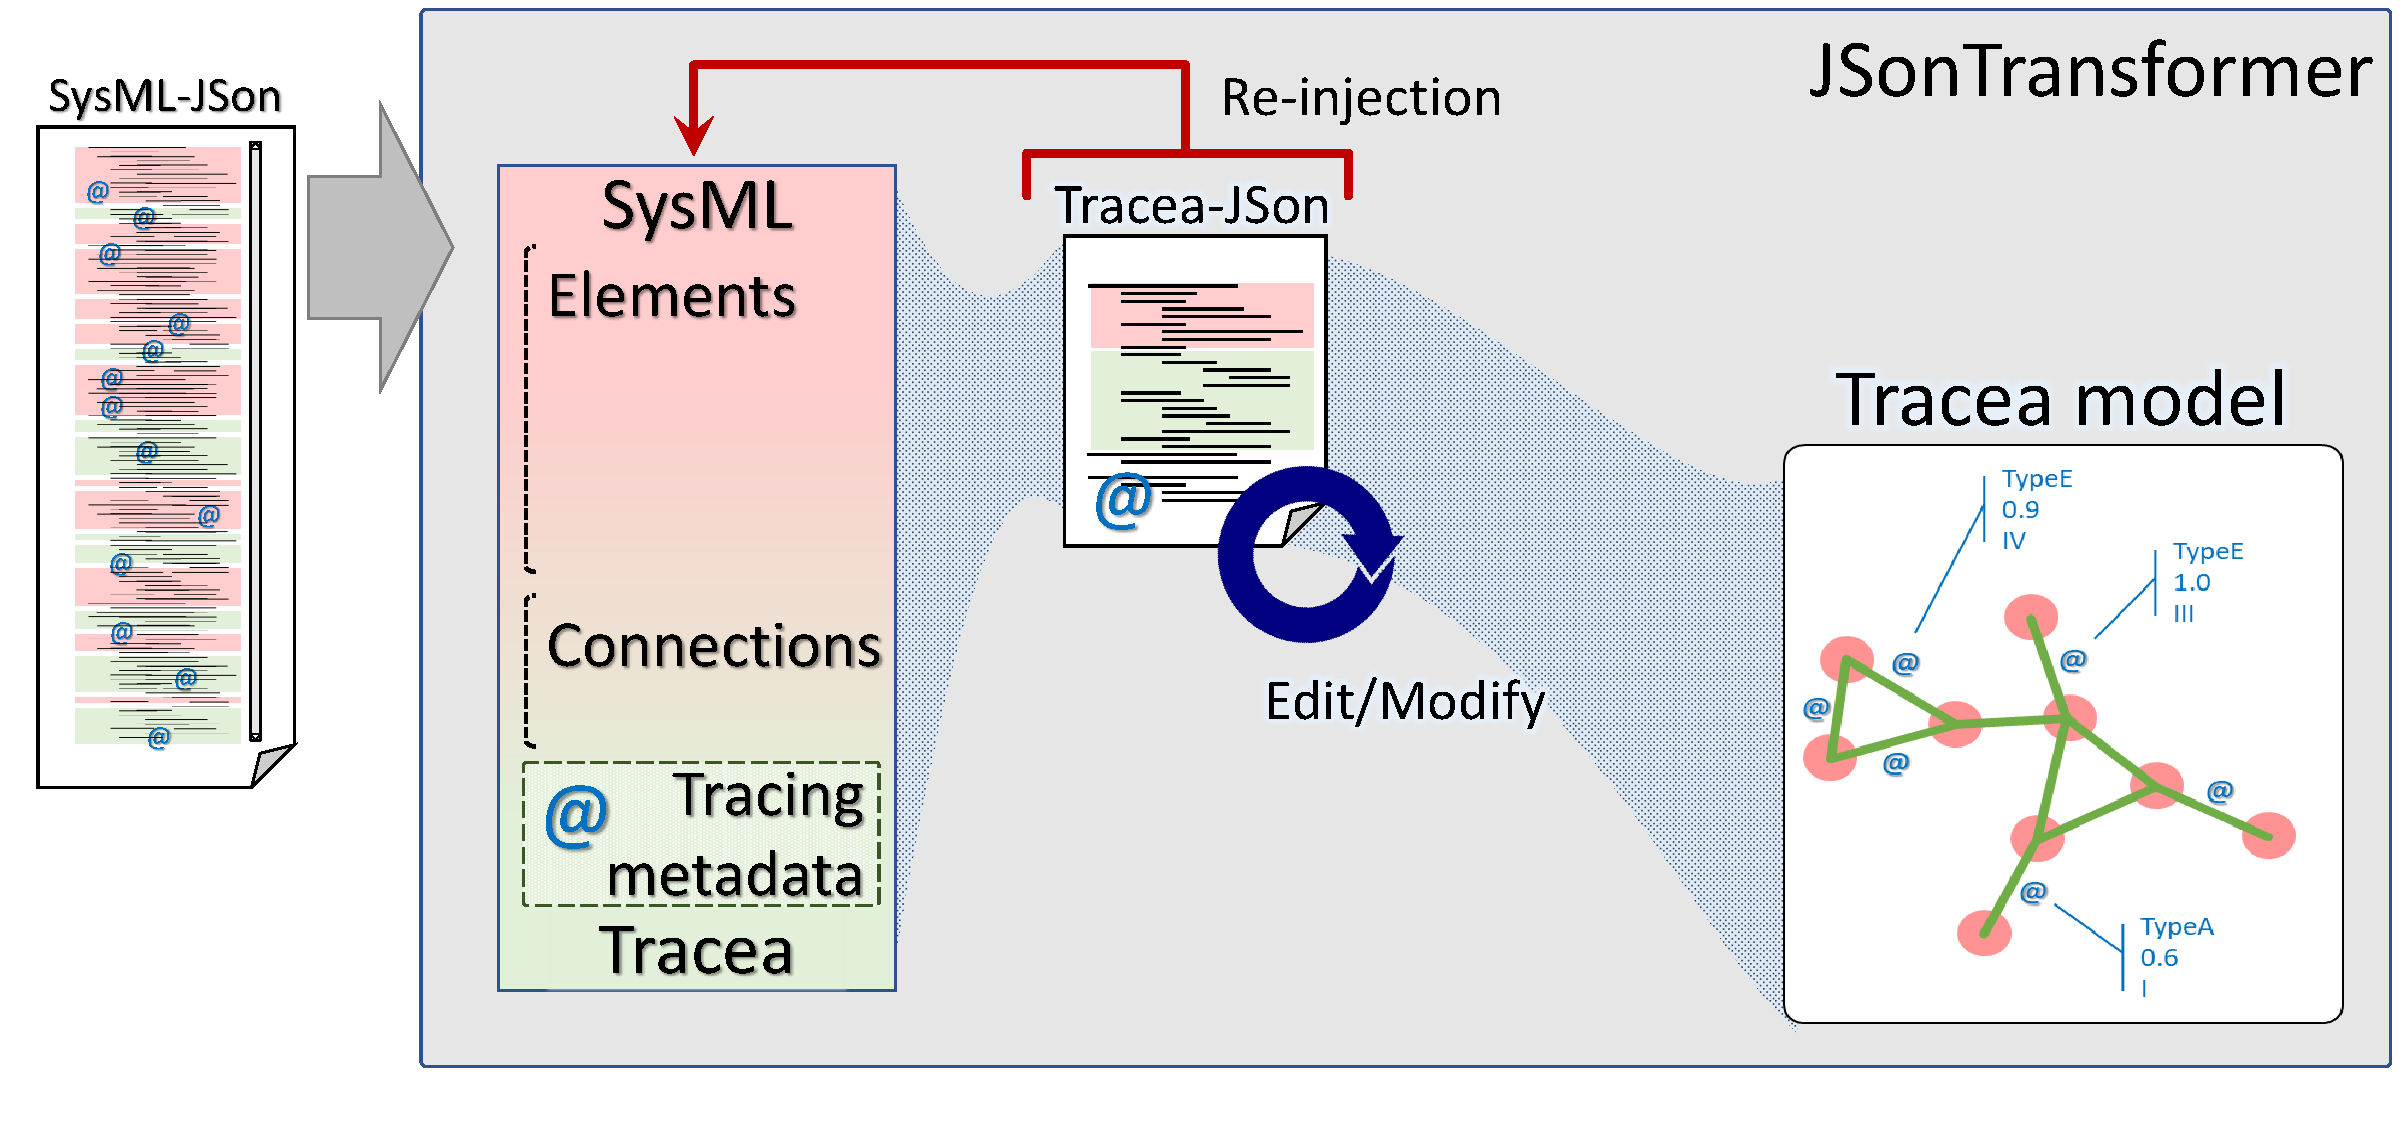
\includegraphics[width=.85\linewidth]{images/JSonTransformer-intern.pdf}
	\caption{JSonTransformer: integration of Tracea with SysMLv2.}
	\label{fig:jsontransformer}
\end{figure}

\Fig{fig:jsontransformer} shows the big picture of the integration of Tracea and SysMLv2 with JSonTransformer\footnote{\url{https://github.com/ebatot/TraceaingJson}}. To remain orthogonal to the system, and to asynch ourselves from the changes in the language itself, we export a JSon snapshots of the SysMLv2 model. Export can be made from the Jupyter implementation or the Eclipse pilot implementation independently. From this very voluble expression of the model (say 50kLoC for a minimalist model of a few elements and a couple of links), we extract a core model to transform and manipulate easily into other format (for more details about Tracea-JSon see Section~\ref{sec:traceamodel}). This format allows the use of multi-end and multi-type links, using the IDs of the elements in the same manner as the original (SysML) file. 

\textit{[Most of the work here lies in the transformation from this raw JSon to the prettied "Tracea" version we target.]}


\subsection{Extraction and re-injection of metadata}

\begin{figure}[ht]
	\centering
	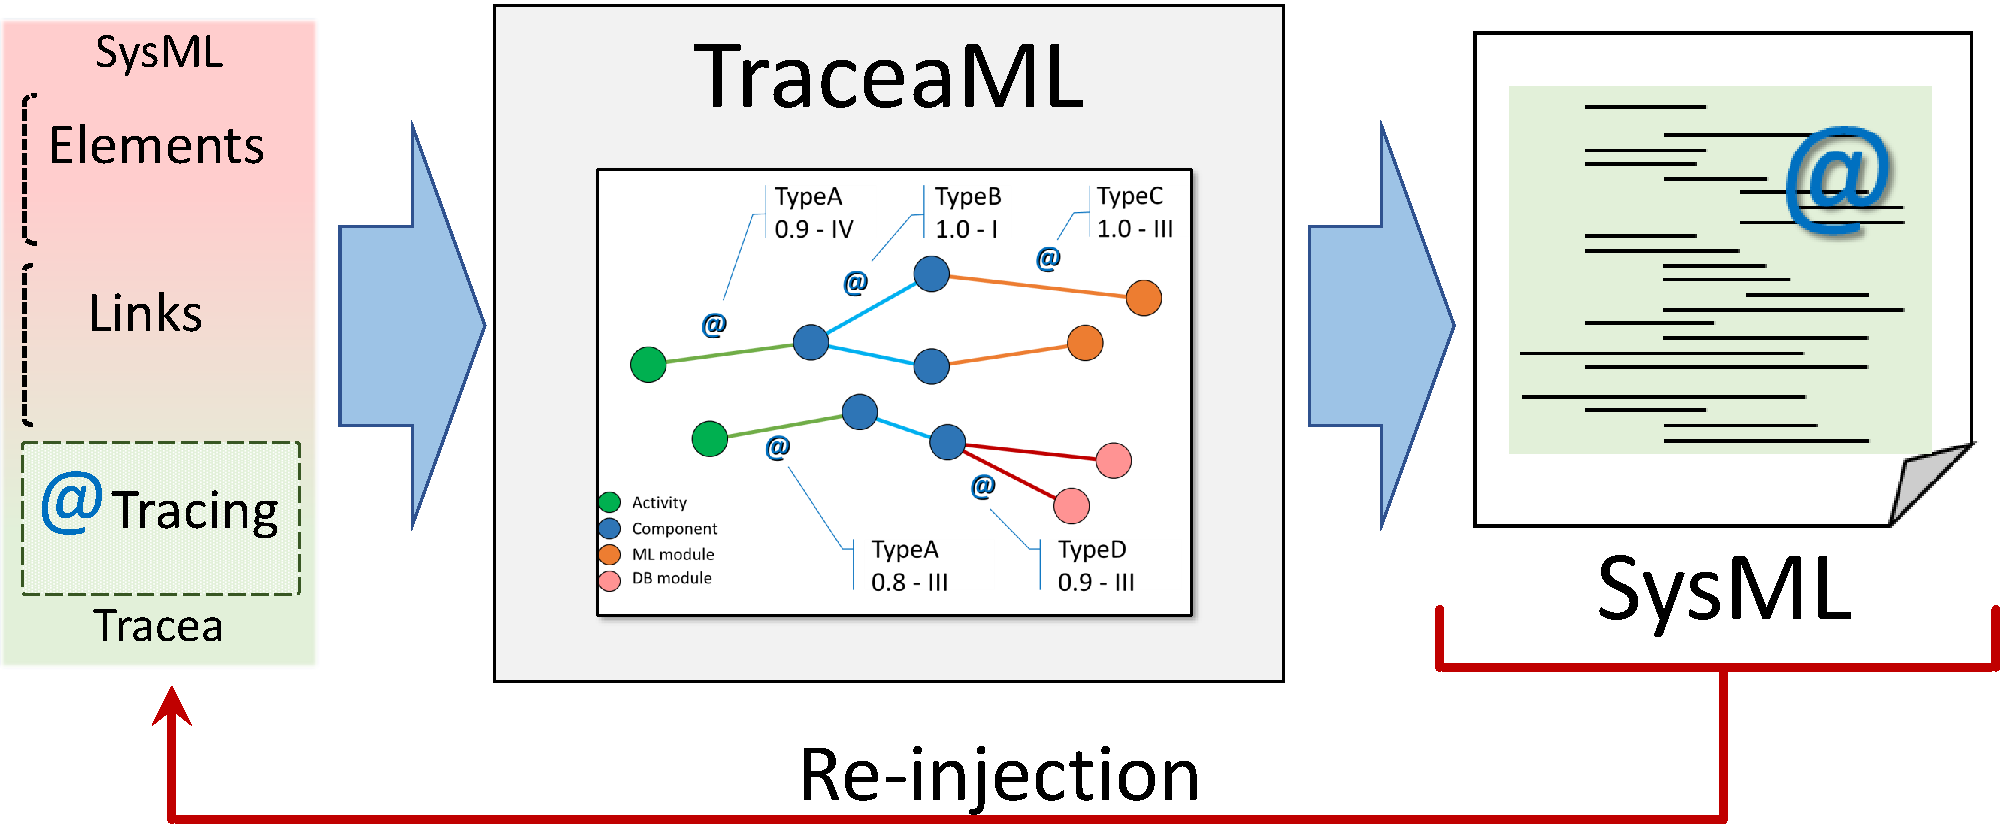
\includegraphics[width=.7\linewidth]{images/reinject.pdf}
	\caption{Re-injection of tracing metadata into a SysML model.}
	\label{fig:reinject}
\end{figure}

Transforming the JSon persistence of the SysMLv2 model comes at a cost. The entire JSon is used as input and our tool extract the necessary information. After editing this information, we re-inject it in the model through a (model-to-text) transformation. We take the \textit{Tracea} model and transform it to SysMLv2 textual notation. 

This method allows us to remain independent from the evolution of the pilot implementation. We act directly on the concrete artefacts -- which in the eyes of the SST is bond to its present version and will not change (\textit{much}) any soon. This method follows a bottom up understanding of the model: we reason from examples (at the instance level) to build and browse the feature paths of interest of the SysMLv2 metamodel. 

\subsection{Implementation details}

\subsubsection{Conditions of use}

Using a JSon snapshot requires that the instances of the links (or \textit{ConnectionUsages} in SysMLv2 terminology) be stored separately, and named. Indeed, metadata is affected to elements through their name. We only target (and source) tracelink with coarse grain elements to avoid the engineering complexity to browse feature paths. 
Summarized:
\begin{itemize}
    \item \textbf{Separated files} -- in order to re-inject the connections and their metadata, these must be kept separated in SysML (textual).
    \item \textbf{Named connections} -- metadata attribution from external source (the keyword "metadata" requires a named target).
    \item \textbf{Coarse grain targets} -- browsing features' path is a coding challenge on its own that is not addressed in the current version of our implementation.
    \item \textbf{External metadata} -- in order to be able to re-inject metadata without collision with existing ones, all metadata must be "external", \textit{i.e.,} declared with "metadata" keyword in SysML.
    \item \textbf{Feature IDs "bug"} -- Identification of SysMLv2 features is buggy: the same feature called from two connections distinct show two IDs. We bypass this limitation using names as identifier for features.
\end{itemize}

\subsubsection{Unexpected SysMLv2 identifier allocation}
As mentioned previously, implementing JSonTransformer, we ran into an unexpected behavior related to the allocation of identifiers to targets and sources of connections. We reported the "bug" to the SST and recorded it in our Git repository at \url{https://github.com/modelia/tracea/tree/master/4-sysml-json-transformer/sysml_id_allocation_bug}

\subsubsection{Programmatic version}

We envision a programmatic version of the current implementation. The use of the API in the pilot implementation has a steep learning curb and we opted in an hybrid version: using the JSon persistence of the models to work on propagation features. This way we work on concrete cases that we can craft to better suit our needs without requiring the actual implementation to be completely finished.

The current implementation will serve as a guide to implement a programmatic version. In this more interactive version, browsing elements will follow the exact same path as the JSon-snapshoted version.

\subsection{Summary}
\ugh{Need text !}
\Fig{fig:traceaml}  
\begin{figure}[h]     
	\centering
	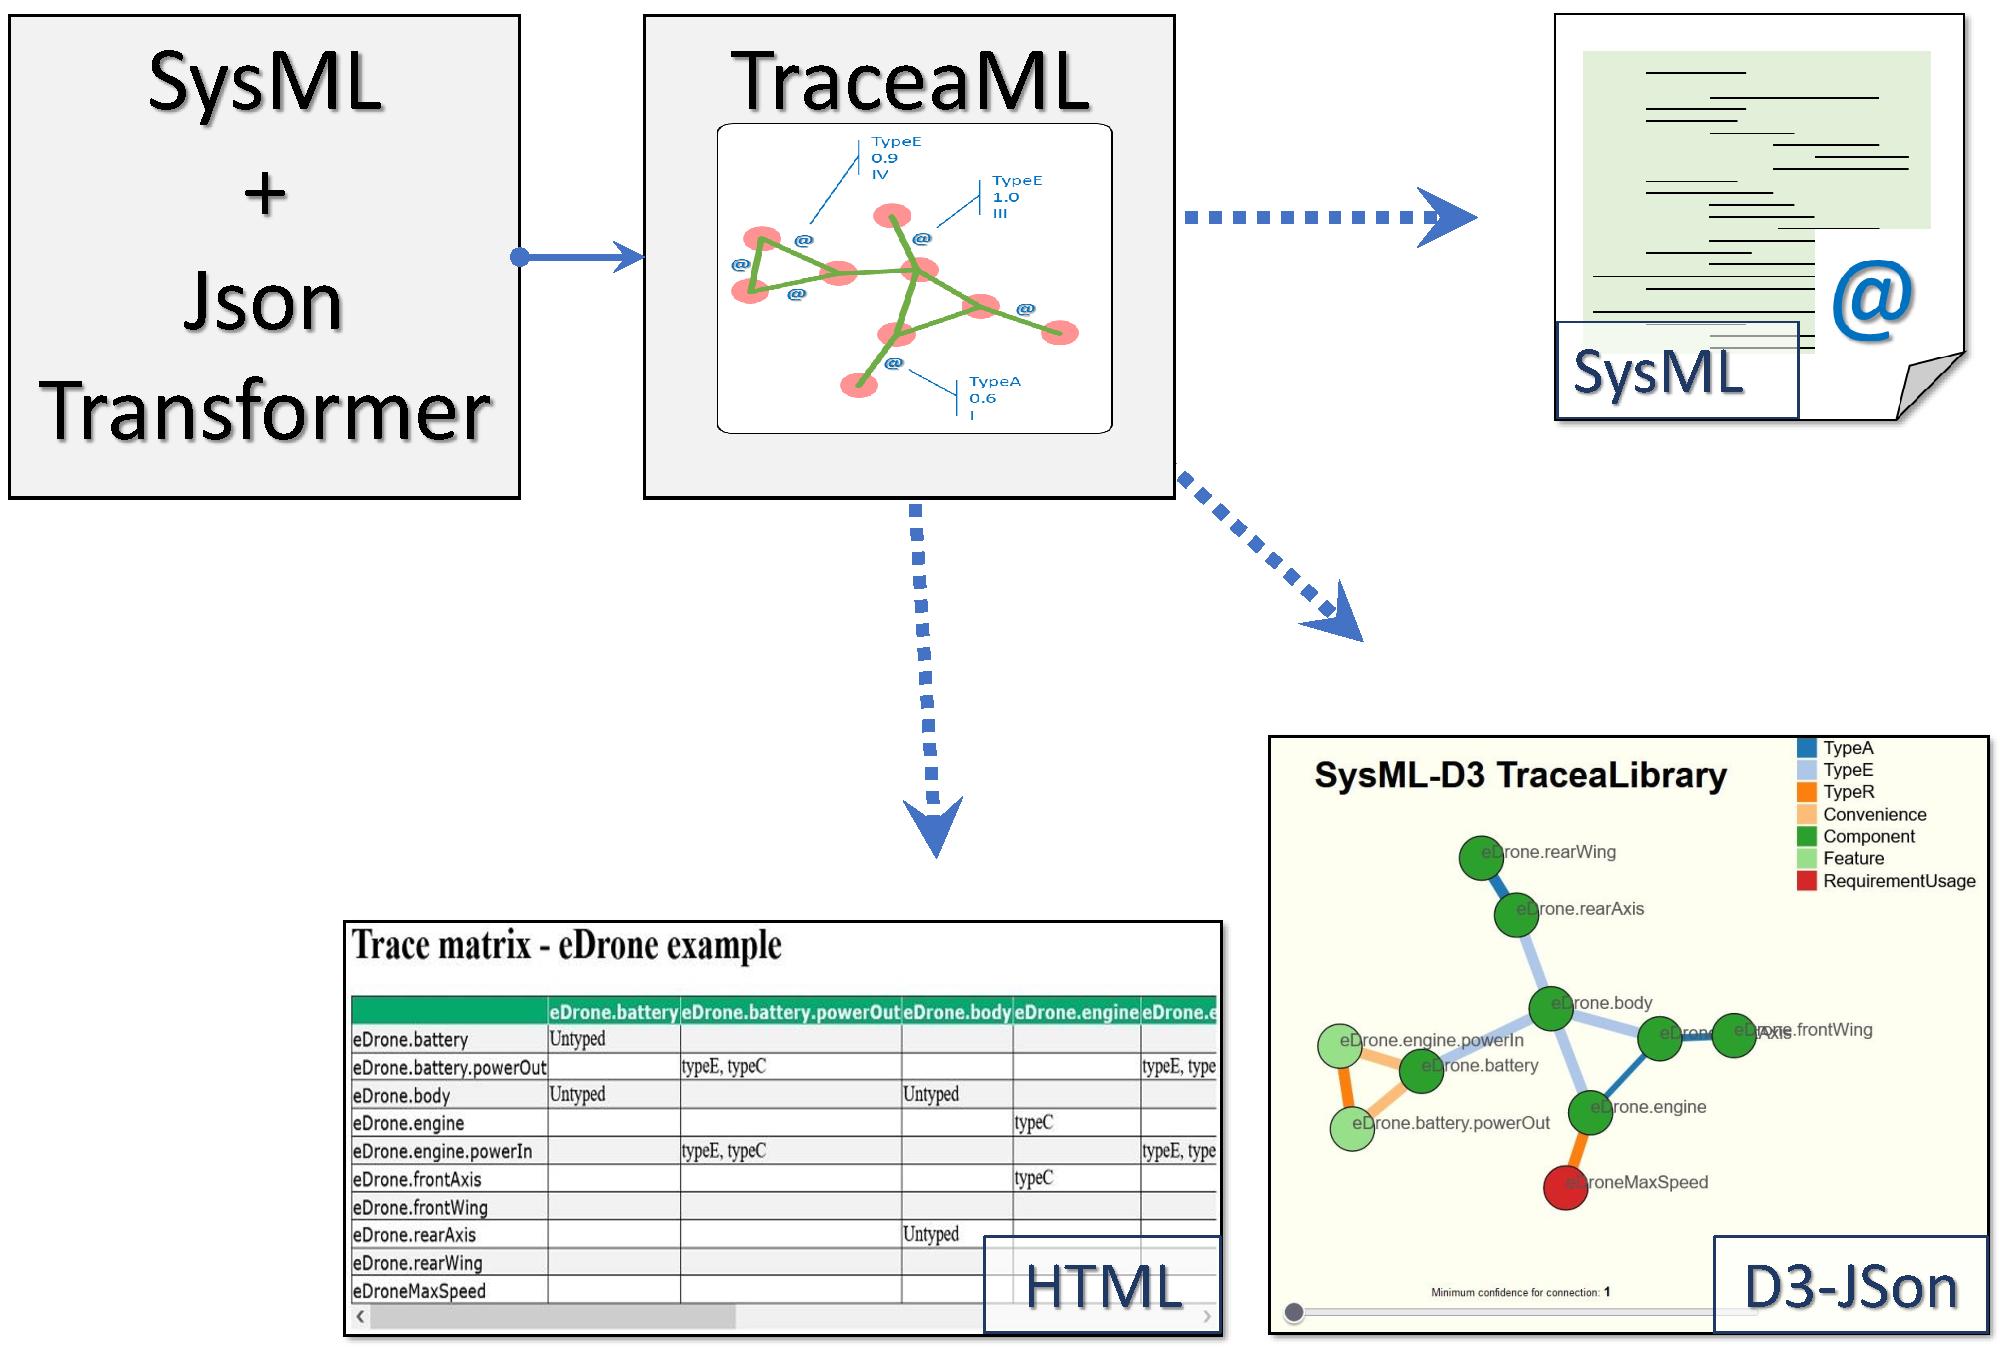
\includegraphics[width=.75\linewidth]{images/traceaml.pdf}
	\caption{SysMLv2 Tracing components, a big picture.}
	\label{fig:traceaml}
\end{figure}
\section{Syntax representation}\label{sec:syntaxrepr}
% \sideboxbegin{o}
% This section presents the limitation encountered while integrating the functionalities of Trace\textit{a} into SysMLv2.
% \sideboxend

In this section we present the different means a user can take a trace to work with. The first version shows a key representation based on Traces's metamodel properties expressed in JSon. The second version is slightly augmented to allow its visualization using the D3-JS API\footnote{\url{https://d3js.org/}}. Last but not least, a matrix-based representation facilitates the analysis of a trace and gives a useful HTML visualization.

\subsection{Trace\textit{a} model}
\label{sec:traceamodel}
\begin{figure}[ht]
	\centering
	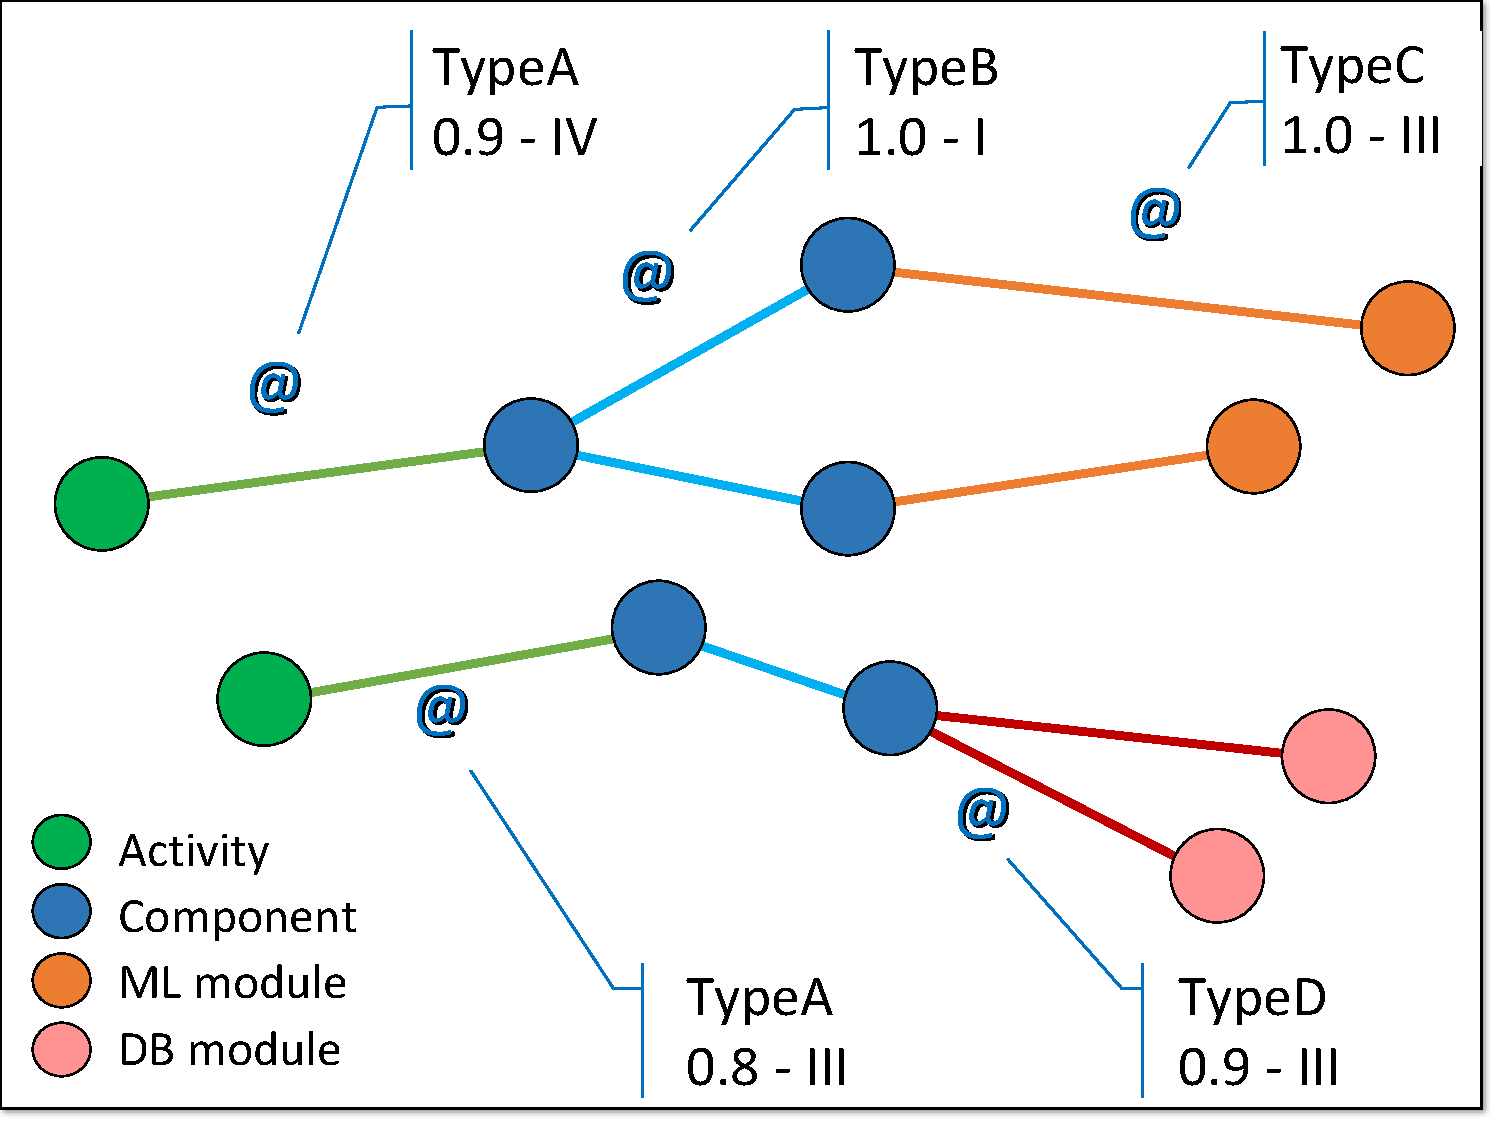
\includegraphics[width=.5\linewidth]{images/energy3.pdf}
	\caption{An illustrative example of a Tracea model.}
	\label{fig:traceamodel}
\end{figure} 
The first representation reflects directly the complex nature of the trace using Trace\textit{a}-like representation. Links are encoded with multiple types and can be multi-ended (source and target alike). This raw representation is the working base for future transformation into specific visualizations, characterized representations, or further mathematical analysis. An illustrative example of a Tracea model is given in \Fig{fig:traceamodel}. Its textual representation is shown in the excerpt of Listing~\ref{lst:traceamodel}.

\begin{center}
\begin{lstlisting}[caption={Excerpt of a trace written in Tracea-JSon.},
label=lst:traceamodel,
style=mystylesysml,
frame=shadowbox,
rulesepcolor=\color{blue},
linewidth=16.6cm,
xleftmargin=0.2cm,
morekeywords={links,id,name,type, source_id, target_id,confidence,nodes,qualifiedName,types,sources,targets}]
{
 "links": [
  { 
    "id": "1085", 
    "name": "eng2front", 
    "qualifiedName": "eDrone_example::eng2front", 
    "types": ["TypeE"], 
    "sources": [{ "id": "b9bb"}],
    "targets": [{ "id": "3adb"}], 
    "confidence": 0.85
  }
   /* ... */
 ], "nodes": [
  { 
    "id": "d83f", 
    "name": "eDrone.battery", 
    "type": "Feature"
  }
  /* ... */
]
}
\end{lstlisting}
\end{center}

\subsection{SysML reinjection}
The Tracea model allows the generation of SysML code to reinject modification, or to populate a model from sources external from the target languages (here SYsML). Listing~\ref{lst:sysmlout} shows a (modified) trace that can be reinjected in the original the model as depicted earlier in \Fig{fig:reinject}.
\begin{center}
\begin{lstlisting}[caption={SysML code generated from a Tracea model.},
label=lst:sysmlout,
style=mystylesysml,
frame=shadowbox,
rulesepcolor=\color{blue},
linewidth=16.6cm,
xleftmargin=0.2cm,
morekeywords={connection,connect,to,metadata,about}]
/* Trace links */
connection eng2front connect eDrone.engine to eDrone.frontAxis;
connection frAx2frWi connect eDrone.frontAxis to eDrone.frontWing;
connection reAx2reWi connect eDrone.rearAxis to eDrone.rearWing;
connection bod2bat connect eDrone.body to eDrone.battery;
connection bod2eng connect eDrone.body to eDrone.engine;
connection bod2frAx connect eDrone.body to eDrone.frontAxis;
connection bod2reAx connect eDrone.body to eDrone.rearAxis;
connection eng2bat_Typed connect eDrone.battery.powerOut to eDrone.engine.powerIn;
connection rq1ToWing connect eDroneMaxSpeed to eDrone.engine;
connection refine1 connect eDrone.battery to eDrone.battery.powerOut;
connection refine2 connect eDrone.battery to eDrone.engine.powerIn;

/* Tracing metadata */
metadata m6093: ConfidenceTracing about eng2front { confidence = 0.85;}
metadata m4103: TraceType about eng2front { tracetype = "TypeE";}
metadata m5096: ConfidenceTracing about frAx2frWi { confidence = 0.65;}
metadata m9040: TraceType about frAx2frWi { tracetype = "TypeE";}
metadata m7556: ConfidenceTracing about reAx2reWi { confidence = 0.75;}
metadata m9270: TraceType about reAx2reWi { tracetype = "TypeE";}
metadata m8202: TraceType about bod2bat { tracetype = "Internal";}
metadata m9711: TraceType about bod2eng { tracetype = "Internal";}
metadata m8159: TraceType about bod2frAx { tracetype = "Internal";}
metadata m7086: TraceType about bod2reAx { tracetype = "Internal";}
metadata m7259: ConfidenceTracing about eng2bat_Typed { confidence = 0.65;}
metadata m3388: TraceType about eng2bat_Typed { tracetype = "TypeA";}
metadata m9094: ConfidenceTracing about rq1ToWing { confidence = 0.45;}
metadata m5621: TraceType about rq1ToWing { tracetype = "TypeA";}
metadata m340: ConfidenceTracing about refine1 { confidence = 0.45;}
metadata m8719: TraceType about refine1 { tracetype = "Convenience";}
metadata m5065: ConfidenceTracing about refine2 { confidence = 0.55;}
metadata m8879: TraceType about refine2 { tracetype = "Convenience";}
\end{lstlisting}
\end{center}

\subsection{Graph visualization}
The literature mention extensively the need for higher level representation to apprehend the inherent complexity of traces. In the end of the day, they are graphs and it sounds of utmost importance to represent them graphically. \Fig{fig:visualizationgraph} shows a graph-based representation of a trace. Each link is an edges between two node-elements. Here, representing multi-ended links is arduous and would require strong decisions. The multi-typed nature of links would need also a further investigation to decide whether to decide the types to show beforehand, or to allow a more interactive manipulation in which there is options to allow users to change them on the fly.

\ugh{Interactivity: confidence/cost thresholds ; tickers for types ; ...}

\begin{figure}[h]
	\centering
	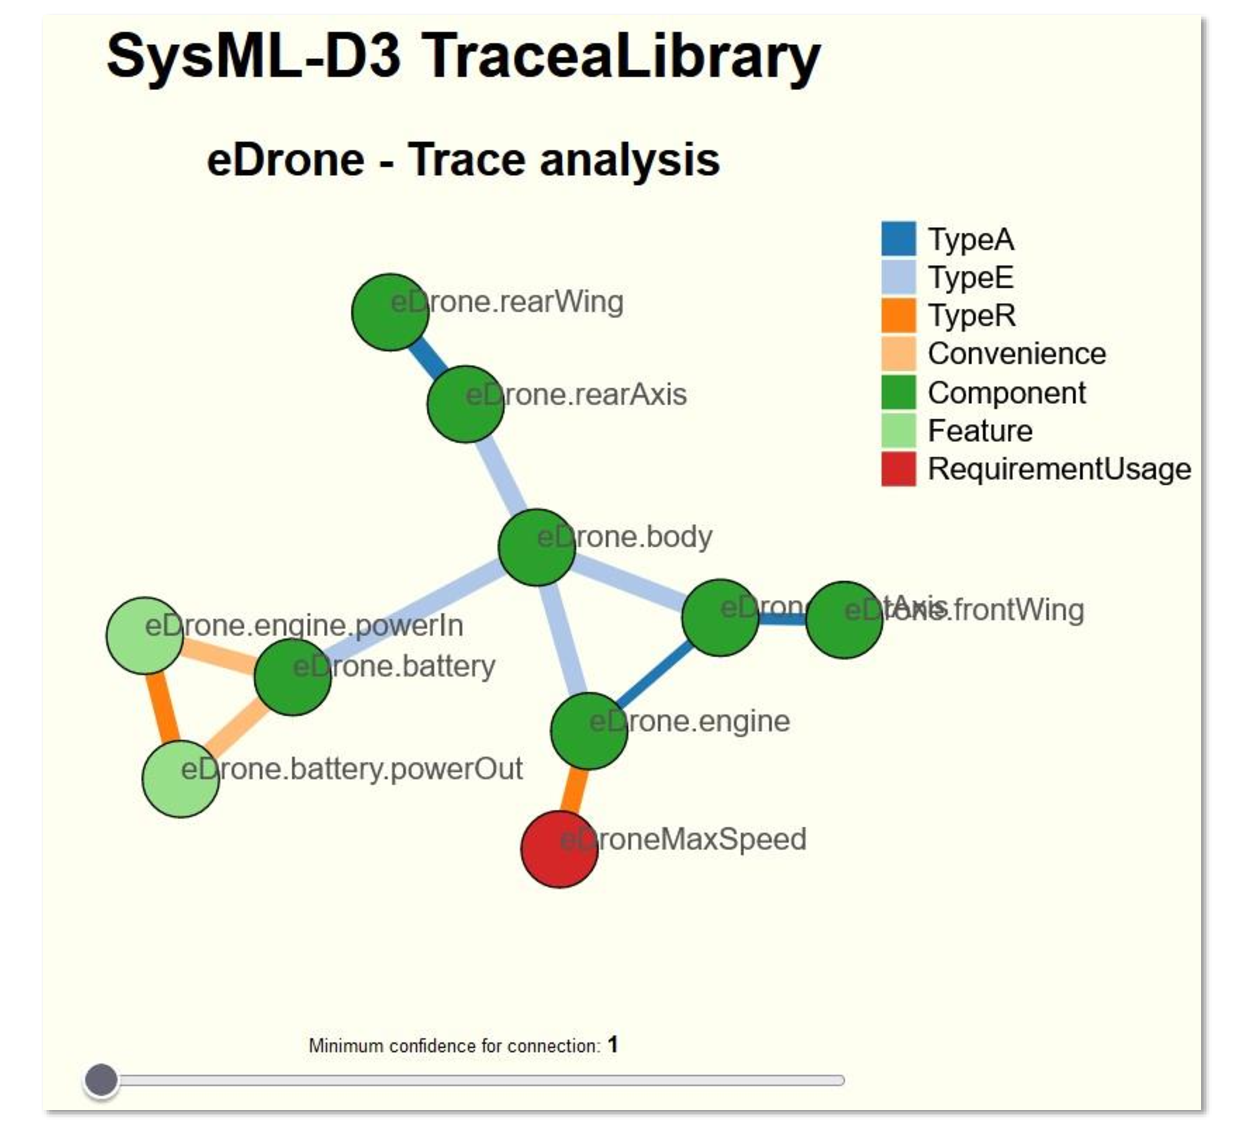
\includegraphics[width=.6\linewidth]{images/visualization1.pdf}
	\caption{A graph-based visualization of a Trace.} 
	\label{fig:visualizationgraph}
\end{figure}

\subsection{Matrix-based view}
Finally, we offer the alternative matrix-based representation of the traces. We export the Trace\textit{a model} as text and HTML tables. The latter is rather interesting. The use of interactive instances of HTML in conjunct use with CSS-JS will allow a valuable set of tools to explore the trace.

\begin{figure}[h]
	\centering
	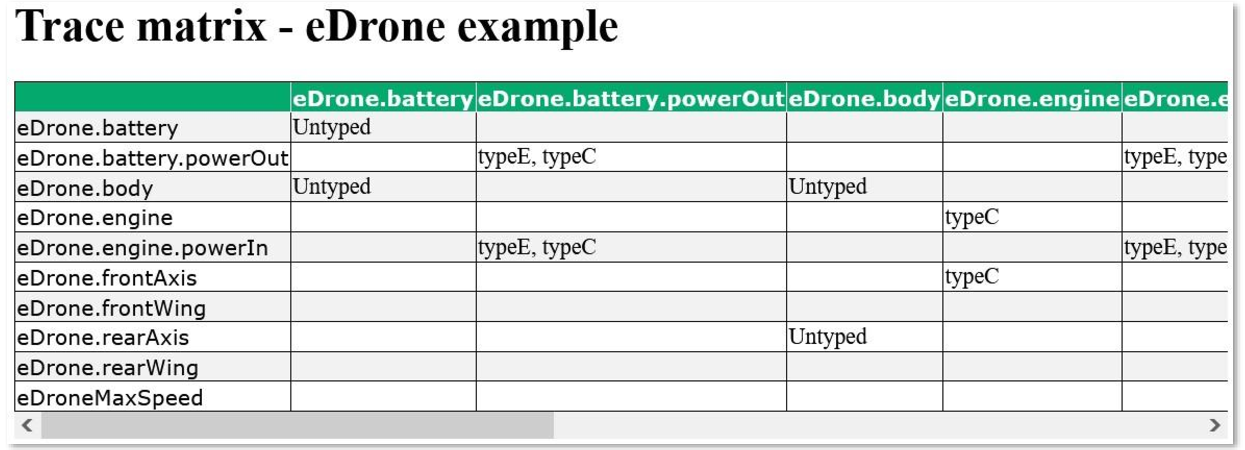
\includegraphics[width=.85\linewidth]{images/matrix1.pdf}
	\caption{A matrix-based representation of a Trace.}
	\label{fig:matrixview}
\end{figure}

\subsection{Interactive features planned}
Using an external tool to handle traces then serves to populate the trace from external sources. In this fashion, an interactive UI shall offer:
\begin{itemize}
    \item To assign trace types to links and define which ones are shown (tickers)
    \item To identify and target ends for links (potentially from a base of tagged elements ?)
    \item To show metadata features (parametered on demand)
    \item To filter links based on thresholds: confidence, cost, energy consumption; or on their type, name, end types...
    \item To export result after manipulation: results of the selection of links / elements, and to export the edited links.
\end{itemize}
 

\section{Implementers' guide}\label{sec:implguide}
% \sideboxbegin{o}
% This section presents the limitation encountered while integrating the functionalities of Trace\textit{a} into SysMLv2.
% \sideboxend



\subsection{Example usage scenario}
\begin{figure}[h]     
	\centering
	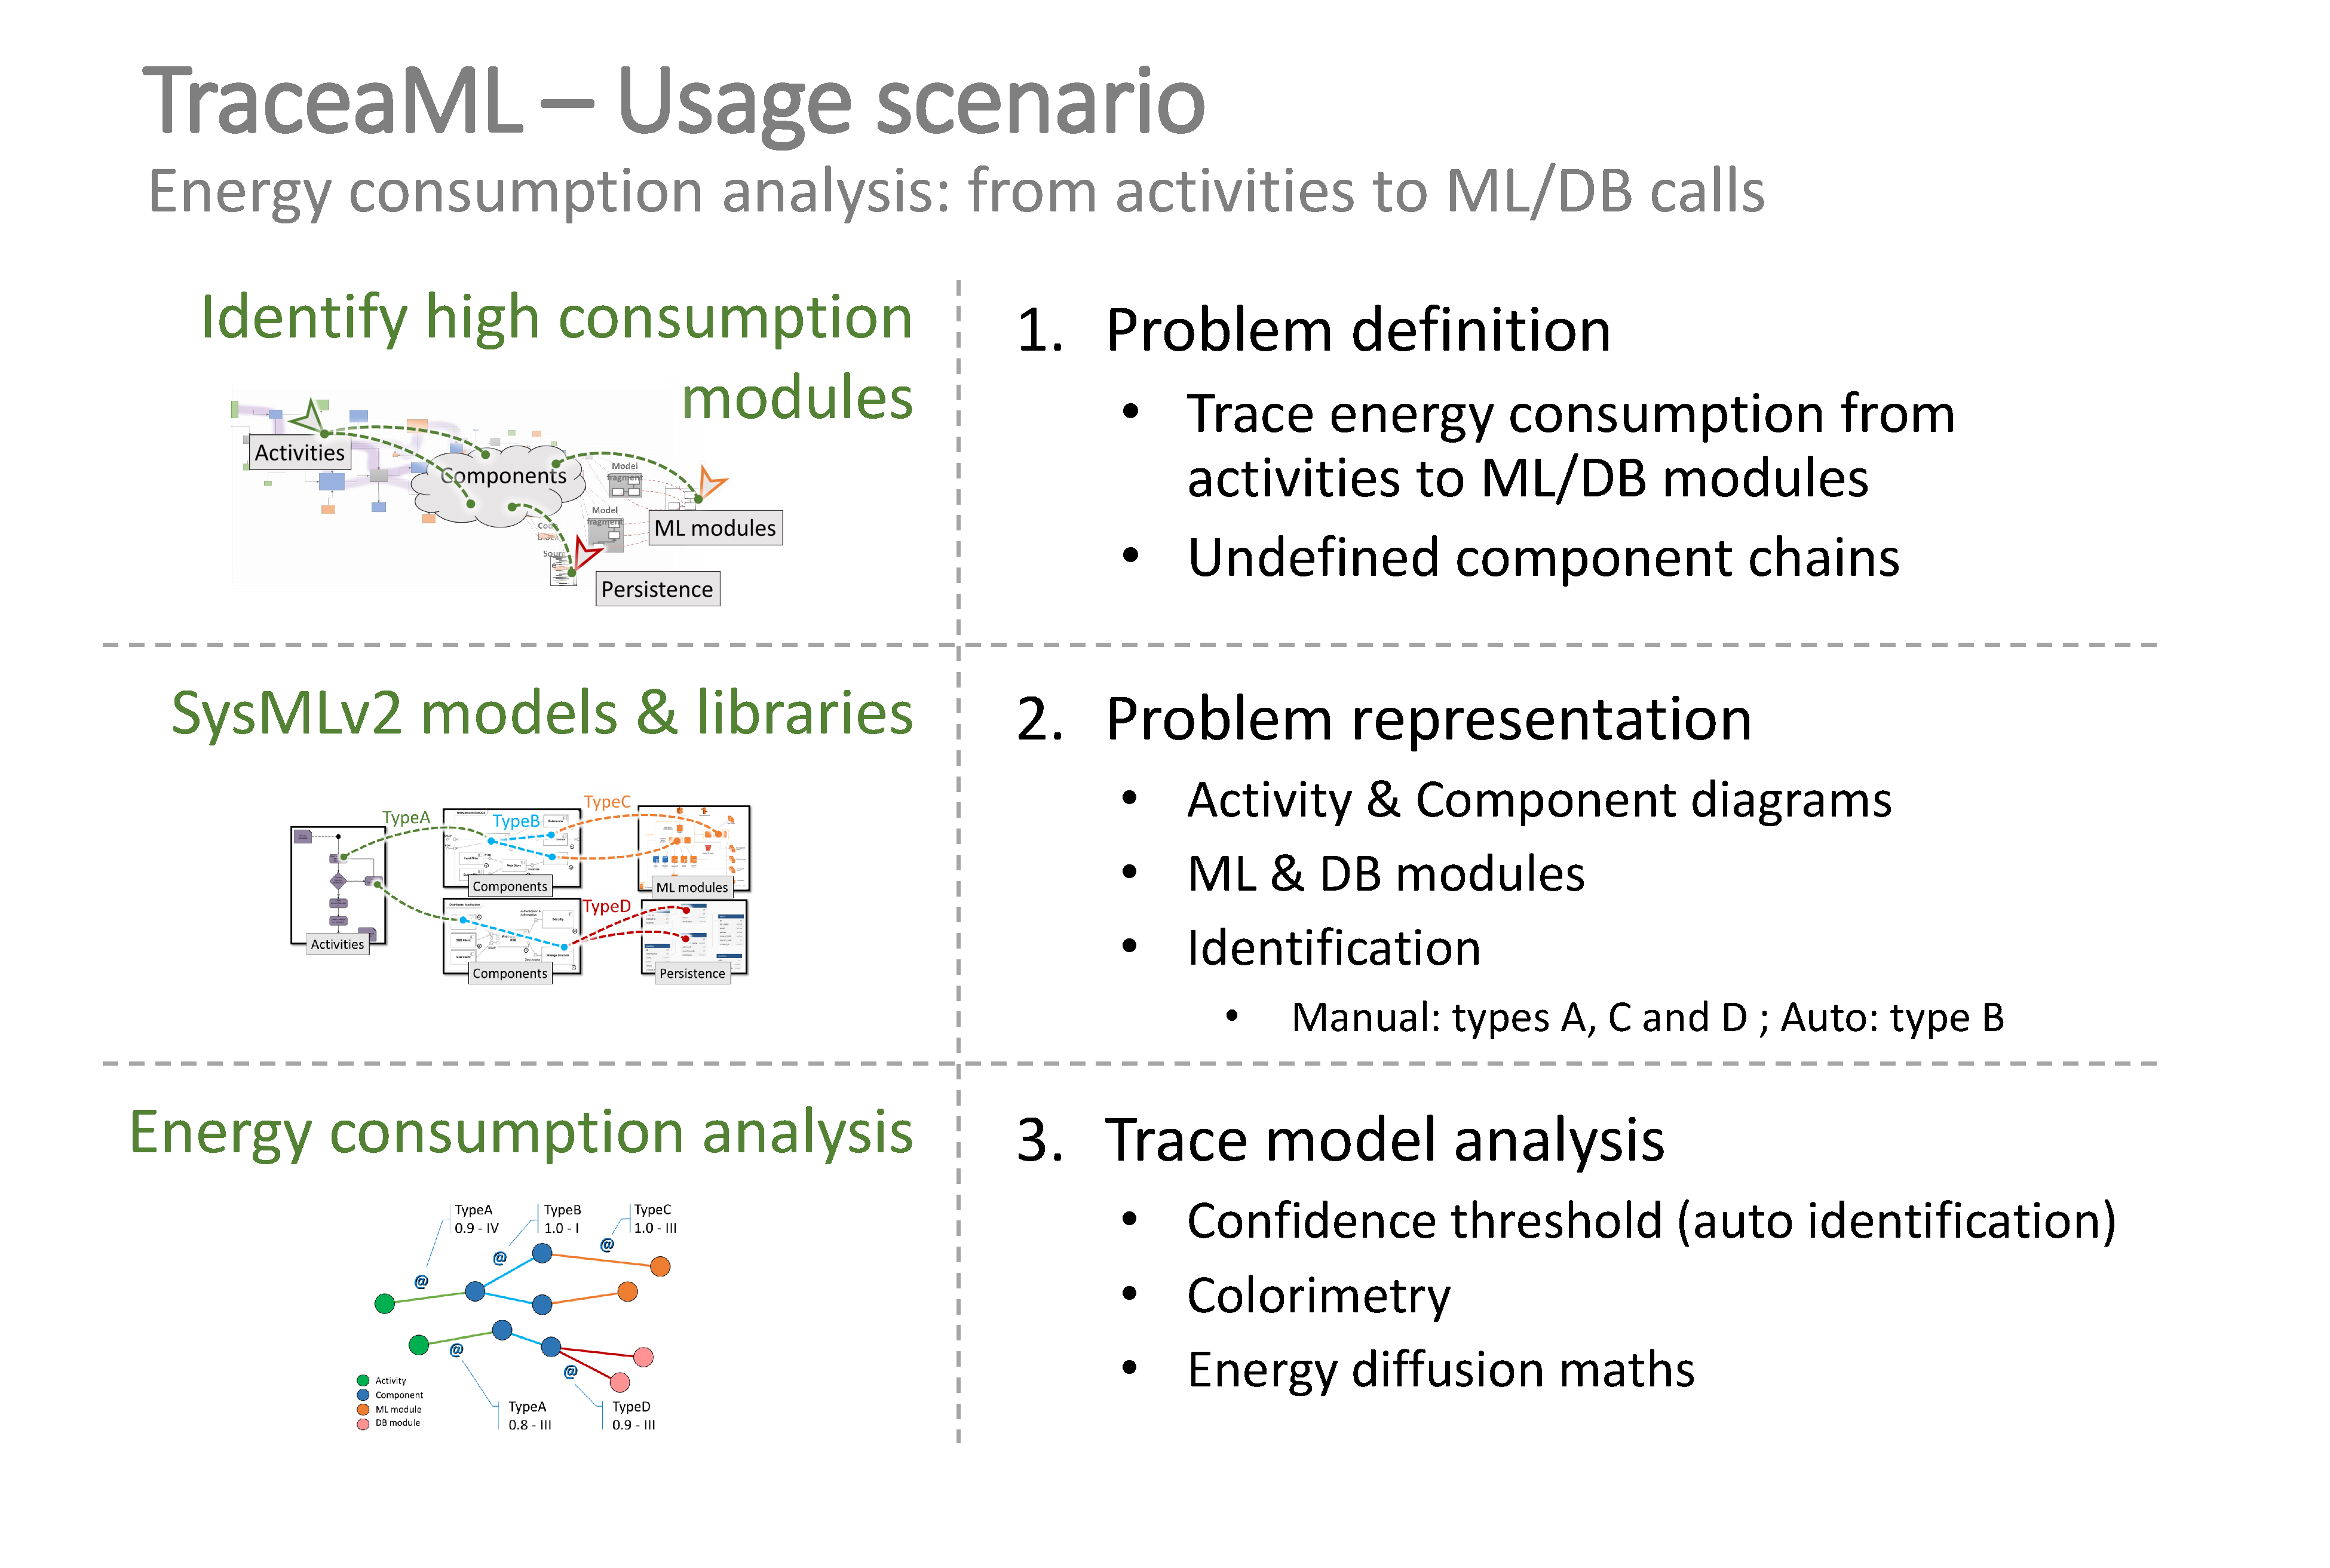
\includegraphics[width=.99\linewidth]{images/scenarionrj.pdf}
	\caption{Use case: Energy consumption analysis.}
	\label{fig:scenarionrj}
\end{figure}


\subsection{Problem definition}
\begin{figure}[h]
	\centering
	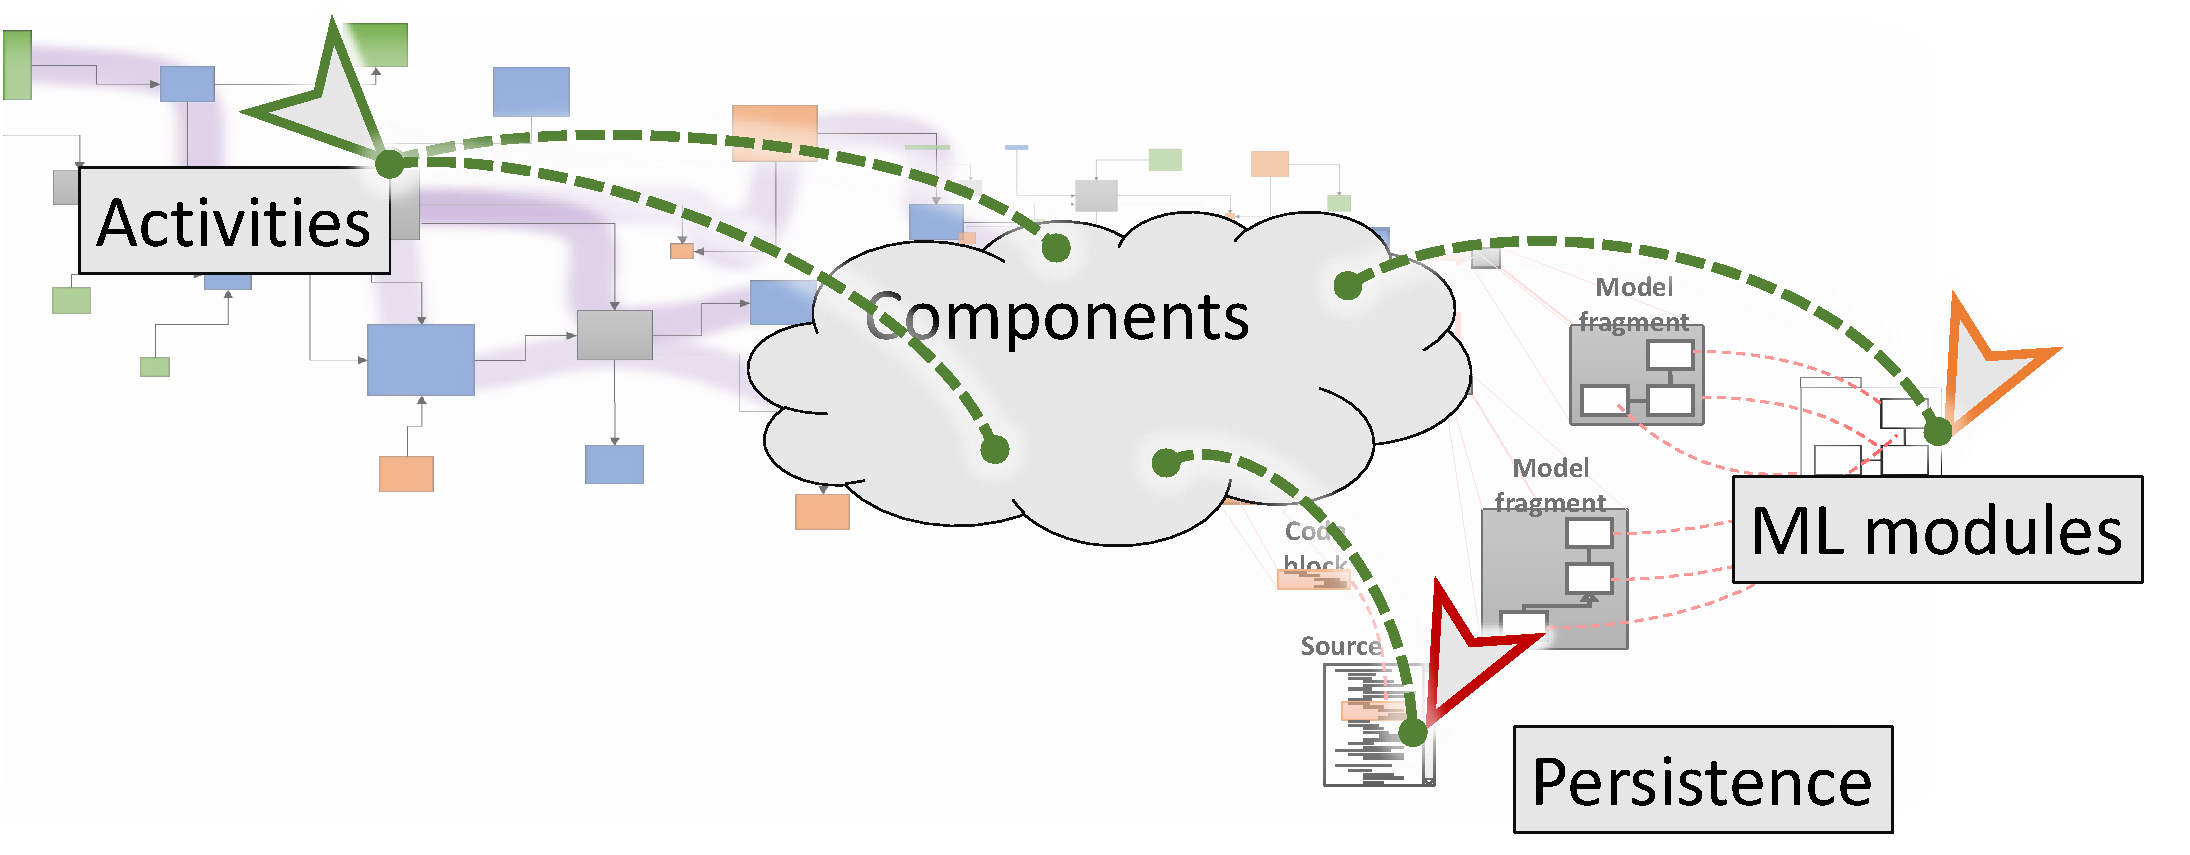
\includegraphics[width=.6\linewidth]{images/energy1.pdf}
	\caption{Problem statement.}
	\label{fig:energy1}
\end{figure}

\subsection{Problem representation}
\begin{figure}[h]     
	\centering
	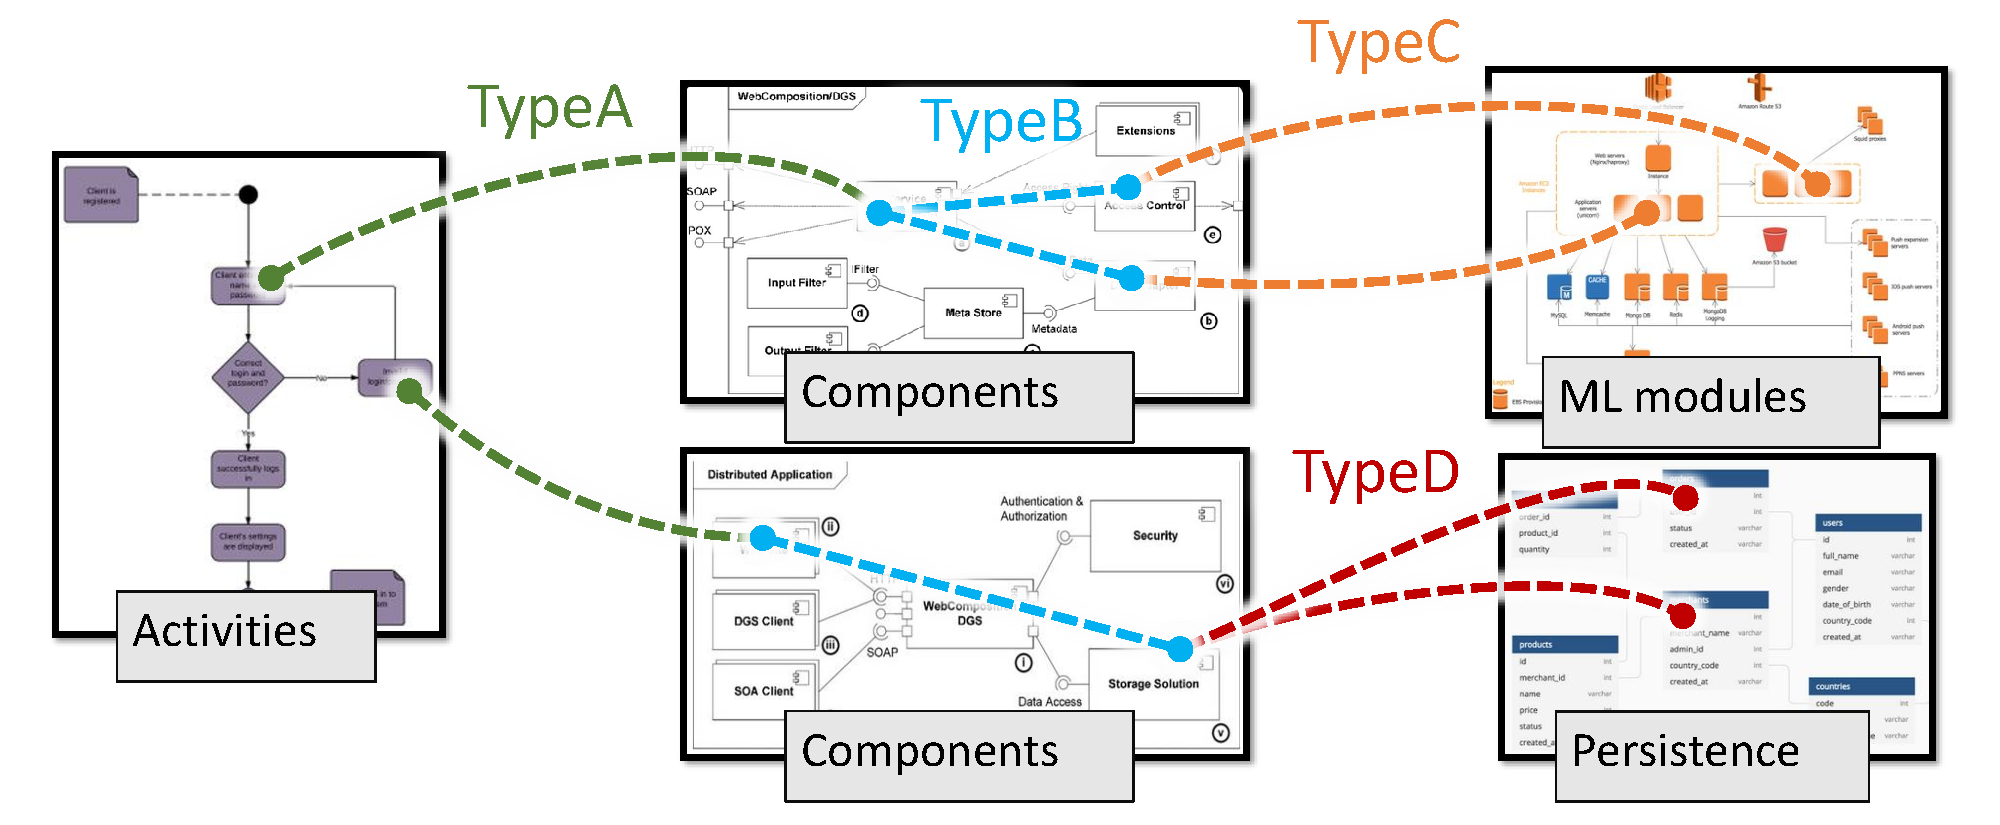
\includegraphics[width=.8\linewidth]{images/energy2.pdf} 
	\caption{Problem representation.}
	\label{fig:energy2}
\end{figure}

\subsection{Trace model analysis}
\begin{figure}[h]     
	\centering
	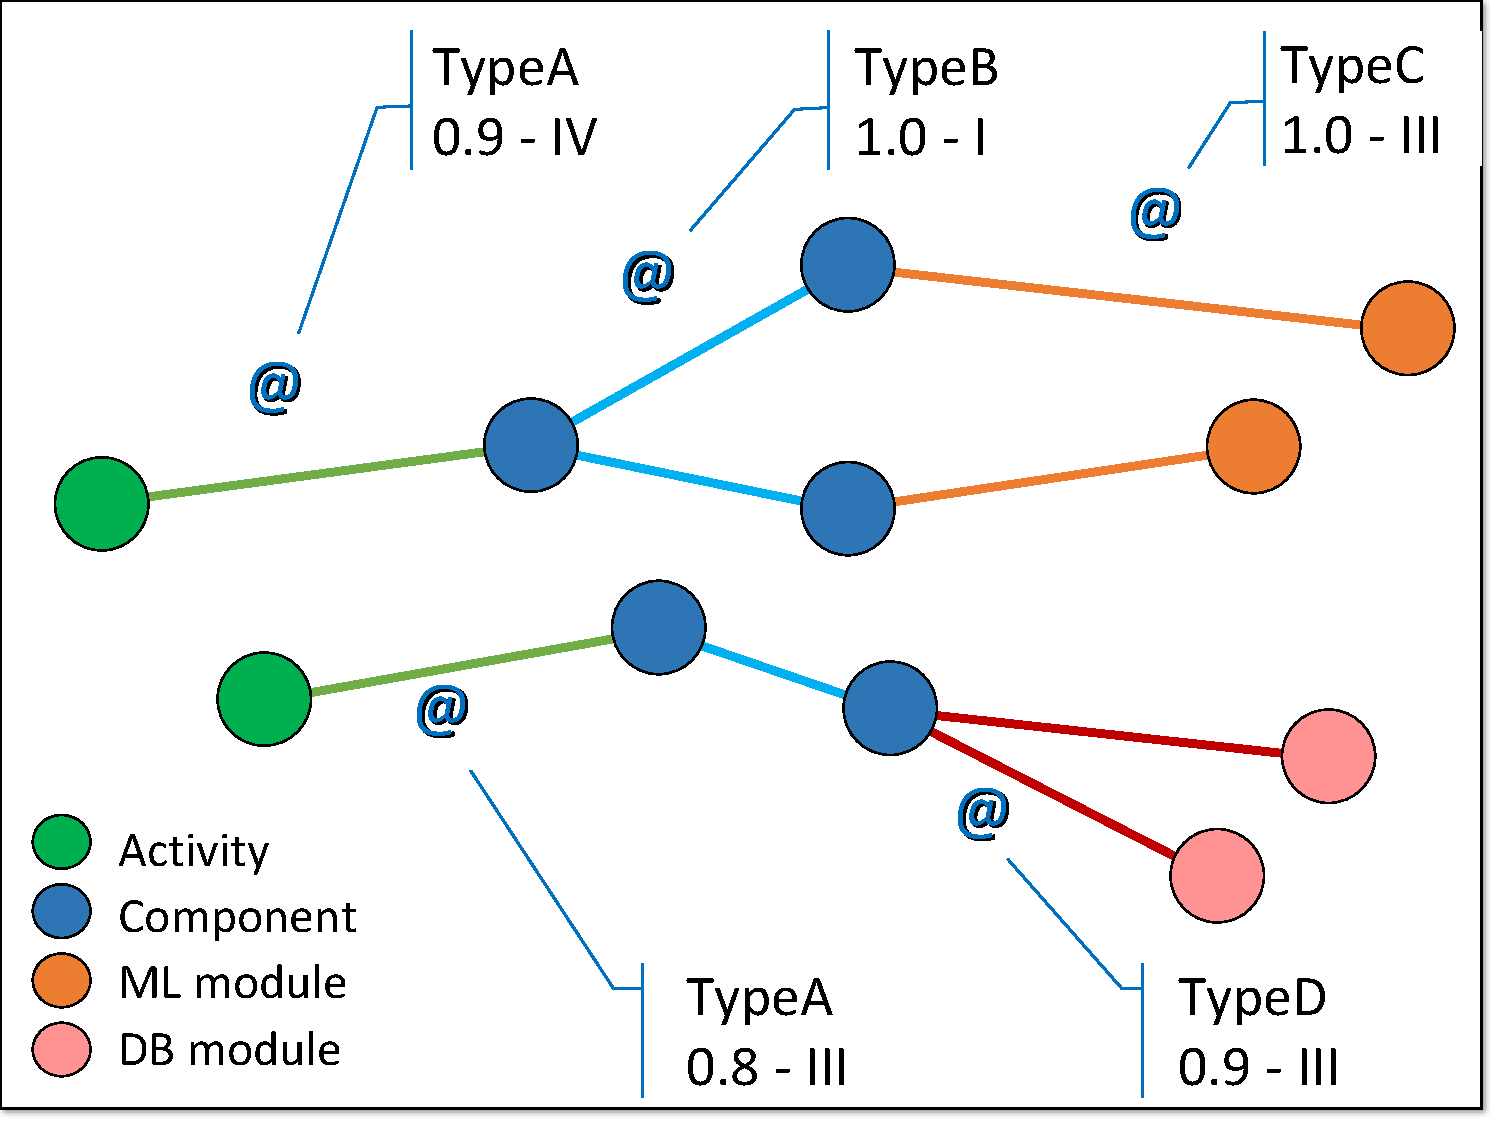
\includegraphics[width=.5\linewidth]{images/energy3.pdf}
	\caption{Trace model representation.}
	\label{fig:energy3}
\end{figure}

\subsection{Toward multi-criteria apprehension}



\section{Conclusion}\label{sec:conclusion}
% \begin{descriptioncompact}
%     \item[Protocol] We propose a protocol to evaluate traceability solution
%     \item[Application] We show an application on Capra.
%     \item[Extension] We detail the extension of Capra as an example of Tracea integration.
%     \item[Limitations] We show Capra's design limitations
% \end{descriptioncompact}
\ugh{D5 - Conclusion !!}
This deliverable presents means to integrate quality traceability into SysMLv2 using Trace\textit{a}.
With Trace\textit{a} datatypes, SysMLv2 relationships can be annotated with valuable information related to their quality -- \textit{i.e.,} their \textit{trustability}. 
The degree of confidence as well as the information necessary to justify it can be associated to SysML links (connections) through metadata definition.


This integration is \textit{orthogonal}. It does not impact the structure of the language itself -- changes happen at the model level with new feature libraries, not at the metamodel level.
This allows the (re)use of the machinery supporting (meta)annotations and eases the (re)definition of tracing structures specific to a certain project or company. We showcase these benefits in one small example that also reveals the current limitations of SysMLv2's implementation.

The SST confirms that annotating features are valuable and salient artefacts in the development of SysML. They shall take more and more importance in the future releases. Work on the evaluation of expressions at the model level is highly required and will be part of the agenda of the fourth quarter of 2021. 
Finally, as a sign of encouragement, the SST invites us to further investigate in the direction we took. 

\section{Software artefacts}\label{sec:artefacts}
The software artifacts we have implemented have been uploaded to the Modelia Git repository and can be accessed at:
\url{https://github.com/modelia/tracea/tree/master/4-sysml-json-transformer}.

The folder contains:
\begin{itemize}
    \item \textbf{TraceaLibrary} in two versions: with trace types as \textit{Strings} and as \textit{Enum literals} ;
    \item An \textbf{example definition}: the definition of an eDrone in SysMLv2: architecture, requirements, definitions, and a set of traces ;
    \item The \textbf{example output} files: JSonTransformer outputs 4 files for the eDrone example, respectively to the four formats mentioned in Section~\ref{sec:syntaxrepr} ;
    \item A \textbf{D3 script} that plots a graphical visualization of Tracea models ;
    \item A \textbf{"bug" record} that depicts of a strange SysMLv2 behavior related to the allocation of IDs to "dot-notation features".
\end{itemize}

This deliverable gave birth to the JSonTransformer\footnote{\url{https://github.com/ebatot/TraceaingJson}}.


%appendix

% \cleardoublepage

% \section{Appendix}
% \includepdf[pages=-]{includepdf/SAM21\_Not\_Yet\_Another\_Metamodel.pdf}
% \label{sec:AppendixPaper}

%\input{sections/aa-appendix}

% Bibliography
%%%%%%%%%%%%%%%%%%%%%%%%%%%%%%%%%%%%%%%%%%%%%%%%%%%%%%%%%%%%%%%%%%%%%%

\cleardoublepage
\bibliographystyle{plain}
\bibliography{bib/strings-abbr,bib/trace-and-models,bib/uoc2020_tracea,bib/added}

% Clarifications
%%%%%%%%%%%%%%%%%%%%%%%%%%%%%%%%%%%%%%%%%%%%%%%%%%%%%%%%%%%%%%%%%%%%%%

% Print them only if the notes package is loaded (c@pagenode exists)
% and there are notes defined within the document (pnotesavechap > 0)

\makeatletter
\ifcsname c@pagenote\endcsname
\ifthenelse{\value{pnotesavechap}>0}{\cleardoublepage\printnotes}{}
\fi
\makeatother

%\makeback

\end{document}          
